\PassOptionsToPackage{unicode=true}{hyperref} % options for packages loaded elsewhere
\PassOptionsToPackage{hyphens}{url}
%
\documentclass[]{article}
\usepackage{lmodern}
\usepackage{amssymb,amsmath}
\usepackage{ifxetex,ifluatex}
\usepackage{fixltx2e} % provides \textsubscript
\ifnum 0\ifxetex 1\fi\ifluatex 1\fi=0 % if pdftex
  \usepackage[T1]{fontenc}
  \usepackage[utf8]{inputenc}
  \usepackage{textcomp} % provides euro and other symbols
\else % if luatex or xelatex
  \usepackage{unicode-math}
  \defaultfontfeatures{Ligatures=TeX,Scale=MatchLowercase}
\fi
% use upquote if available, for straight quotes in verbatim environments
\IfFileExists{upquote.sty}{\usepackage{upquote}}{}
% use microtype if available
\IfFileExists{microtype.sty}{%
\usepackage[]{microtype}
\UseMicrotypeSet[protrusion]{basicmath} % disable protrusion for tt fonts
}{}
\IfFileExists{parskip.sty}{%
\usepackage{parskip}
}{% else
\setlength{\parindent}{0pt}
\setlength{\parskip}{6pt plus 2pt minus 1pt}
}
\usepackage{hyperref}
\hypersetup{
            pdftitle={Analisis de Muchos Modelos},
            pdfauthor={Sebastian Jaremczuk},
            pdfborder={0 0 0},
            breaklinks=true}
\urlstyle{same}  % don't use monospace font for urls
\usepackage[margin=1in]{geometry}
\usepackage{listings}
\newcommand{\passthrough}[1]{#1}
\usepackage{graphicx,grffile}
\makeatletter
\def\maxwidth{\ifdim\Gin@nat@width>\linewidth\linewidth\else\Gin@nat@width\fi}
\def\maxheight{\ifdim\Gin@nat@height>\textheight\textheight\else\Gin@nat@height\fi}
\makeatother
% Scale images if necessary, so that they will not overflow the page
% margins by default, and it is still possible to overwrite the defaults
% using explicit options in \includegraphics[width, height, ...]{}
\setkeys{Gin}{width=\maxwidth,height=\maxheight,keepaspectratio}
\setlength{\emergencystretch}{3em}  % prevent overfull lines
\providecommand{\tightlist}{%
  \setlength{\itemsep}{0pt}\setlength{\parskip}{0pt}}
\setcounter{secnumdepth}{0}
% Redefines (sub)paragraphs to behave more like sections
\ifx\paragraph\undefined\else
\let\oldparagraph\paragraph
\renewcommand{\paragraph}[1]{\oldparagraph{#1}\mbox{}}
\fi
\ifx\subparagraph\undefined\else
\let\oldsubparagraph\subparagraph
\renewcommand{\subparagraph}[1]{\oldsubparagraph{#1}\mbox{}}
\fi

% set default figure placement to htbp
\makeatletter
\def\fps@figure{htbp}
\makeatother

\usepackage{booktabs}
\usepackage{longtable}
\usepackage{array}
\usepackage{multirow}
\usepackage{wrapfig}
\usepackage{float}
\usepackage{colortbl}
\usepackage{pdflscape}
\usepackage{tabu}
\usepackage{threeparttable}
\usepackage{threeparttablex}
\usepackage[normalem]{ulem}
\usepackage{makecell}
\usepackage{xcolor}

\title{Analisis de Muchos Modelos}
\author{Sebastian Jaremczuk}
\date{2020-04-17}

\begin{document}
\maketitle

\hypertarget{carga-de-datos}{%
\subsubsection{carga de datos}\label{carga-de-datos}}

\hypertarget{knn}{%
\section{KNN}\label{knn}}

\hypertarget{modelar}{%
\subsection{Modelar}\label{modelar}}

El modelo obtenido durante el entrenamiento es el siguiente:

\begin{lstlisting}
## k-Nearest Neighbors 
## 
## 3191 samples
##   24 predictor
##    2 classes: '0', '1' 
## 
## No pre-processing
## Resampling: Cross-Validated (10 fold, repeated 5 times) 
## Summary of sample sizes: 2872, 2872, 2872, 2872, 2872, 2872, ... 
## Resampling results across tuning parameters:
## 
##   k   Accuracy   Kappa    
##    1  0.7583203  0.5077784
##    2  0.7535556  0.4981009
##    5  0.7956132  0.5810591
##   10  0.7993774  0.5877563
##   15  0.8021971  0.5937258
##   20  0.8033252  0.5959767
##   30  0.8049545  0.5995533
##   50  0.8124159  0.6144606
##   60  0.8122281  0.6140509
##   70  0.8127294  0.6149712
##   80  0.8096591  0.6085439
## 
## Accuracy was used to select the optimal model using the largest value.
## The final value used for the model was k = 70.
\end{lstlisting}

\begin{table}[!h]

\caption{\label{tab:kmeans_2_resumen}Resumen composición de cluster Kmeans según clase desertor}
\centering
\begin{tabular}[t]{rrrrr}
\toprule
\rowcolor{black}  \multicolumn{1}{c}{\textcolor{white}{\textbf{k}}} & \multicolumn{1}{c}{\textcolor{white}{\textbf{Accuracy}}} & \multicolumn{1}{c}{\textcolor{white}{\textbf{Kappa}}} & \multicolumn{1}{c}{\textcolor{white}{\textbf{AccuracySD}}} & \multicolumn{1}{c}{\textcolor{white}{\textbf{KappaSD}}}\\
\midrule
\rowcolor{gray!6}  1 & 0.7583203 & 0.5077784 & 0.0218490 & 0.0451777\\
2 & 0.7535556 & 0.4981009 & 0.0216224 & 0.0439617\\
\rowcolor{gray!6}  5 & 0.7956132 & 0.5810591 & 0.0202191 & 0.0417847\\
10 & 0.7993774 & 0.5877563 & 0.0228967 & 0.0477935\\
\rowcolor{gray!6}  15 & 0.8021971 & 0.5937258 & 0.0229241 & 0.0476222\\
\addlinespace
20 & 0.8033252 & 0.5959767 & 0.0204760 & 0.0428055\\
\rowcolor{gray!6}  30 & 0.8049545 & 0.5995533 & 0.0209553 & 0.0434628\\
50 & 0.8124159 & 0.6144606 & 0.0209855 & 0.0437144\\
\rowcolor{gray!6}  60 & 0.8122281 & 0.6140509 & 0.0206854 & 0.0430537\\
70 & 0.8127294 & 0.6149712 & 0.0209825 & 0.0437856\\
\addlinespace
\rowcolor{gray!6}  80 & 0.8096591 & 0.6085439 & 0.0224092 & 0.0466400\\
\bottomrule
\end{tabular}
\end{table}

\begin{lstlisting}
##     k
## 10 70
\end{lstlisting}

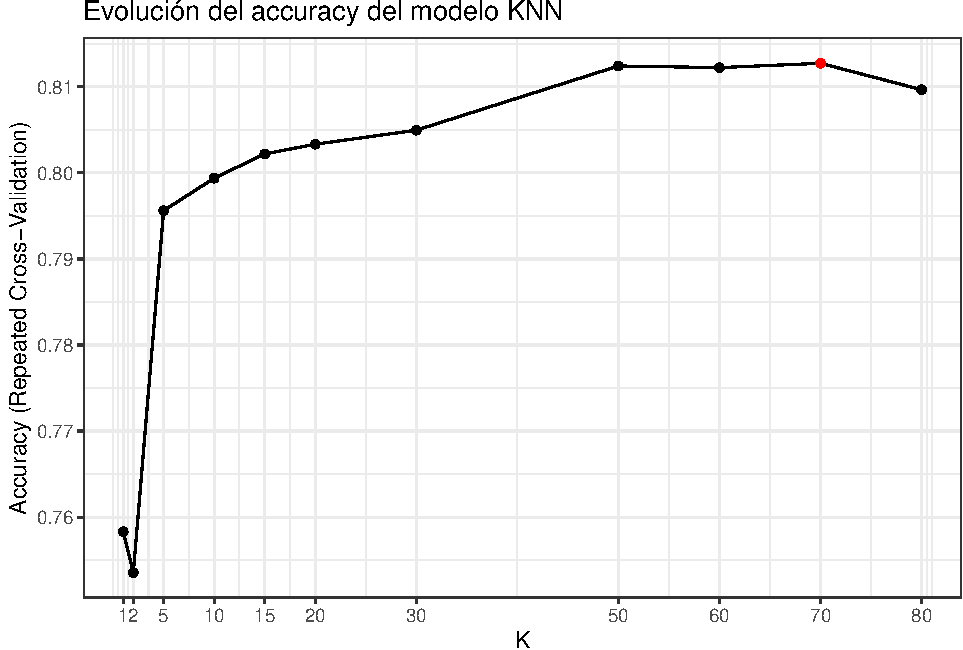
\includegraphics{analisis_de_muchos_modelos_files/figure-latex/unnamed-chunk-13-1.pdf}

Se puede decir que el mejor modelo obtenido en la etapa de entrenamiento
es con k = 70 con un accuracy promedio de 81,27 \%

\hypertarget{describir-el-modelo}{%
\subsection{describir el modelo}\label{describir-el-modelo}}

El modelo de knn entrenado aporta un buen porcentaje de aciertos que
supera ampliamente el nivel mínimo que corresponde a la clase
mayoritaria. Sin embargo, una mejor manera de avaluarlo es utilizando el
conjunto de test cuyas observaciones no han sido utilizadas hasta ahora.

\begin{table}[!h]

\caption{\label{tab:MatrizConf_KNN}Matriz de Confusion del metodo: KNN }
\centering
\begin{tabular}[t]{lcc}
\toprule
\multicolumn{1}{c}{Prediccion} & \multicolumn{1}{c}{Referencia} & \multicolumn{1}{c}{ } \\
\cmidrule(l{3pt}r{3pt}){1-1} \cmidrule(l{3pt}r{3pt}){2-2}
\rowcolor{black}  \multicolumn{1}{c}{\textcolor{white}{\textbf{ }}} & \multicolumn{1}{c}{\textcolor{white}{\textbf{0}}} & \multicolumn{1}{c}{\textcolor{white}{\textbf{1}}}\\
\midrule
\rowcolor{gray!6}  0 & 657 & 160\\
1 & 110 & 440\\
\bottomrule
\end{tabular}
\end{table}

\begin{table}[!h]

\caption{\label{tab:metricas_KNN}Métricas del metodo: KNN }
\centering
\begin{tabular}[t]{cc}
\toprule
\rowcolor{black}  \multicolumn{1}{c}{\textcolor{white}{\textbf{metricas}}} & \multicolumn{1}{c}{\textcolor{white}{\textbf{valor}}}\\
\midrule
\rowcolor{gray!6}  Accuracy & 0.8024872\\
Kappa & 0.5953182\\
\rowcolor{gray!6}  AccuracyLower & 0.7803760\\
AccuracyUpper & 0.8232897\\
\rowcolor{gray!6}  AccuracyNull & 0.5610827\\
\addlinespace
AccuracyPValue & 0.0000000\\
\rowcolor{gray!6}  McnemarPValue & 0.0028633\\
Sensitivity & 0.7333333\\
\rowcolor{gray!6}  Specificity & 0.8565841\\
Pos Pred Value & 0.8000000\\
\addlinespace
\rowcolor{gray!6}  Neg Pred Value & 0.8041616\\
Precision & 0.8000000\\
\rowcolor{gray!6}  Recall & 0.7333333\\
F1 & 0.7652174\\
\rowcolor{gray!6}  Prevalence & 0.4389173\\
\addlinespace
Detection Rate & 0.3218727\\
\rowcolor{gray!6}  Detection Prevalence & 0.4023409\\
Balanced Accuracy & 0.7949587\\
\bottomrule
\end{tabular}
\end{table}

Como es de esperarse, los aciertos en el dataset de Test son menores que
en el de entrenamiento. En este caso un 80.3 \% el cual sigue siendo muy
bueno y se encuentra por encima del nivel mínimo que corresponde a la
clase maypritaria (56\%)

\hypertarget{naive-bayes}{%
\section{Naive Bayes}\label{naive-bayes}}

Este algoritmo calcula las probabilidades condicionales de que una
observación pertenezca a cada una de las clases según los valores de los
predictores. El algoritmo asume que las variables son independientes. De
esta forma, se puede calcular la probabilidad cuando hay múltiples
predictores multiplicando las probabilidades individuales de cada uno ya
que se asume que son eventos independientes.

\hypertarget{determinar-parametros-del-modelo}{%
\subsection{determinar Parametros del
modelo}\label{determinar-parametros-del-modelo}}

Aquí existen 3 parámetros:

\begin{itemize}
\item
  usekernel: se asigna FALSE para asumir una distribución de densidad
  gaussiana. Si fuera TRUE, se debería emplear un kernel para estimar la
  densidad.
\item
  fL: factor de corrección de Laplace, 0 para no aplicar ninguna
  corrección. En este caso no aplicaremos corrección.
\item
  adjust: 0 si usekernel es FALSE. Si usekernel es TRUE se completa con
  el parámetro correspondiente para la función density.
\end{itemize}

\hypertarget{modelar-1}{%
\subsection{Modelar}\label{modelar-1}}

Durante el entrenamiento, el mejor ajuste fue con un 76.44\% en Accuracy

\begin{lstlisting}
## Naive Bayes 
## 
## 3191 samples
##   24 predictor
##    2 classes: '0', '1' 
## 
## No pre-processing
## Resampling: Cross-Validated (10 fold, repeated 5 times) 
## Summary of sample sizes: 2872, 2872, 2872, 2872, 2872, 2872, ... 
## Resampling results:
## 
##   Accuracy   Kappa    
##   0.7644649  0.5344009
## 
## Tuning parameter 'fL' was held constant at a value of 0
## Tuning
##  parameter 'usekernel' was held constant at a value of FALSE
## Tuning
##  parameter 'adjust' was held constant at a value of 0
\end{lstlisting}

\hypertarget{describir-el-modelo-1}{%
\subsection{Describir el modelo}\label{describir-el-modelo-1}}

Este modelo aparentemente es ligeramente menos efectivo que el KNN visto
anteriormente. Para una evluación correcta, se realizan las predicciones
sobre el datasets de test, arrojando los siguientes resultados:

\begin{table}[!h]

\caption{\label{tab:MatrizConf_KNN}Matriz de Confusion del metodo: KNN }
\centering
\begin{tabular}[t]{lcc}
\toprule
\multicolumn{1}{c}{Prediccion} & \multicolumn{1}{c}{Referencia} & \multicolumn{1}{c}{ } \\
\cmidrule(l{3pt}r{3pt}){1-1} \cmidrule(l{3pt}r{3pt}){2-2}
\rowcolor{black}  \multicolumn{1}{c}{\textcolor{white}{\textbf{ }}} & \multicolumn{1}{c}{\textcolor{white}{\textbf{0}}} & \multicolumn{1}{c}{\textcolor{white}{\textbf{1}}}\\
\midrule
\rowcolor{gray!6}  0 & 657 & 160\\
1 & 110 & 440\\
\bottomrule
\end{tabular}
\end{table}

\begin{table}[!h]

\caption{\label{tab:metricas_KNN}Métricas del metodo: KNN }
\centering
\begin{tabular}[t]{cc}
\toprule
\rowcolor{black}  \multicolumn{1}{c}{\textcolor{white}{\textbf{metricas}}} & \multicolumn{1}{c}{\textcolor{white}{\textbf{valor}}}\\
\midrule
\rowcolor{gray!6}  Accuracy & 0.8024872\\
Kappa & 0.5953182\\
\rowcolor{gray!6}  AccuracyLower & 0.7803760\\
AccuracyUpper & 0.8232897\\
\rowcolor{gray!6}  AccuracyNull & 0.5610827\\
\addlinespace
AccuracyPValue & 0.0000000\\
\rowcolor{gray!6}  McnemarPValue & 0.0028633\\
Sensitivity & 0.7333333\\
\rowcolor{gray!6}  Specificity & 0.8565841\\
Pos Pred Value & 0.8000000\\
\addlinespace
\rowcolor{gray!6}  Neg Pred Value & 0.8041616\\
Precision & 0.8000000\\
\rowcolor{gray!6}  Recall & 0.7333333\\
F1 & 0.7652174\\
\rowcolor{gray!6}  Prevalence & 0.4389173\\
\addlinespace
Detection Rate & 0.3218727\\
\rowcolor{gray!6}  Detection Prevalence & 0.4023409\\
Balanced Accuracy & 0.7949587\\
\bottomrule
\end{tabular}
\end{table}

\hypertarget{regresiuxf3n-loguxedstica}{%
\section{Regresión Logística}\label{regresiuxf3n-loguxedstica}}

permite estimar la probabilidad de una variable cualitativa binaria en
función de una variable cuantitativa. Es un algoritmo que puede explicar
bien la respuesta en función de sus predictores. La relación como lo
dice su nombre es logarítmica, por lo que la relación entre las
probabilidades y las variables o es lineal. El incremente en 1 unidad de
una variable depende también del valor que tiene la variable en ese
moemnto (es decir, la posición en la curva logarítmica donde se
encuentra).

\hypertarget{determinar-paruxe1metros}{%
\subsection{Determinar parámetros}\label{determinar-paruxe1metros}}

No existen hiperparámetros. Como en este caso se utiliza el paquete glm,
hay que determinar que se realiza una una regresión logística indicando
que el paquete utilice la familia binomial.

\hypertarget{modelar-2}{%
\subsection{Modelar}\label{modelar-2}}

Con la misma metodología que los modelos anteriores, durante el
entrenamiento este modelo da como resultado un 83.7\% de Accurac, el
cual es muy prometedor. Ademas de estimar buen resultado, este modelo
puede explicar el comportamiento de la variable respuesta en función de
los predictores.

Puede observarse que no todas las variables son significativas, lo que
nos lleva a pensar en el aporte de la misma información por mas de una
variable.

\begin{lstlisting}
## Generalized Linear Model 
## 
## 3191 samples
##   24 predictor
##    2 classes: '0', '1' 
## 
## No pre-processing
## Resampling: Cross-Validated (10 fold, repeated 5 times) 
## Summary of sample sizes: 2872, 2872, 2872, 2872, 2872, 2872, ... 
## Resampling results:
## 
##   Accuracy   Kappa    
##   0.8370451  0.6640431
\end{lstlisting}

\begin{lstlisting}
## 
## Call:
## NULL
## 
## Deviance Residuals: 
##     Min       1Q   Median       3Q      Max  
## -4.6987  -0.5650  -0.2177   0.2764   2.9822  
## 
## Coefficients: (1 not defined because of singularities)
##                                    Estimate Std. Error z value Pr(>|z|)    
## (Intercept)                         0.19916    0.17002   1.171 0.241425    
## Turno_Manana                       -0.11839    0.08164  -1.450 0.147049    
## tipo_de_aprobacion_libre            0.25795    0.06929   3.723 0.000197 ***
## tipo_de_aprobacion_cambio_curso    -0.03145    0.05751  -0.547 0.584462    
## tipo_de_aprobacion_promociono      -0.56523    0.73182  -0.772 0.439902    
## edad_al_ingreso                     0.05958    0.06363   0.936 0.349063    
## tipo_de_aprobacion_no_firmo        -0.14436    0.16954  -0.852 0.394488    
## ciclo_lectivo_de_cursada           -3.00698    0.18112 -16.602  < 2e-16 ***
## tipo_de_aprobacion_firmo           -2.66744    0.35457  -7.523 5.36e-14 ***
## cant_resursada_regular              0.17558    0.06226   2.820 0.004799 ** 
## cant_recursada_regular_No_Recurso   2.98696    0.35175   8.492  < 2e-16 ***
## cant_recursada_regular_Recurso1vez  0.87215    0.13298   6.558 5.44e-11 ***
## cant_recursada_regular_Recurso2vez  0.45362    0.10201   4.447 8.71e-06 ***
## cant_recursada_regular_Recurso3vez  0.33130    0.08042   4.119 3.80e-05 ***
## cant_recursada_regular_Recurso4vez  0.31818    0.07013   4.537 5.71e-06 ***
## Turno_Tarde                        -0.09447    0.06197  -1.524 0.127394    
## Turno_Noche                              NA         NA      NA       NA    
## Aprobado                           -0.77000    0.22058  -3.491 0.000482 ***
## Promociono                         -0.21699    0.72904  -0.298 0.765984    
## noAprobado                         -0.18922    0.09432  -2.006 0.044835 *  
## Nota                                0.23356    0.19245   1.214 0.224882    
## Nota_max_prom                      -0.04499    0.18072  -0.249 0.803380    
## EsTecnico_X1                        0.01100    0.12912   0.085 0.932087    
## EsTecnico_SinDato                   0.54663    0.19660   2.780 0.005428 ** 
## Sexo_M                              0.04451    0.15903   0.280 0.779542    
## ---
## Signif. codes:  0 '***' 0.001 '**' 0.01 '*' 0.05 '.' 0.1 ' ' 1
## 
## (Dispersion parameter for binomial family taken to be 1)
## 
##     Null deviance: 4375.6  on 3190  degrees of freedom
## Residual deviance: 2214.3  on 3167  degrees of freedom
## AIC: 2262.3
## 
## Number of Fisher Scoring iterations: 7
\end{lstlisting}

\hypertarget{describir-el-modelo-2}{%
\subsection{Describir el modelo}\label{describir-el-modelo-2}}

Se evalua el modelo entrenado con el conjunto de Test. En este caso, se
puede observar que el modelo resulta ser bastante robusto obteniendo
casi el mismo valor en Accuracy que el modelo entrenado, 83,54\%. Es un
buen modelo para tener en cuenta y analizarlo mas en profundidad.

\begin{table}[!h]

\caption{\label{tab:MatrizConf_logistic}Matriz de Confusion del metodo: logistic }
\centering
\begin{tabular}[t]{lcc}
\toprule
\multicolumn{1}{c}{Prediccion} & \multicolumn{1}{c}{Referencia} & \multicolumn{1}{c}{ } \\
\cmidrule(l{3pt}r{3pt}){1-1} \cmidrule(l{3pt}r{3pt}){2-2}
\rowcolor{black}  \multicolumn{1}{c}{\textcolor{white}{\textbf{ }}} & \multicolumn{1}{c}{\textcolor{white}{\textbf{0}}} & \multicolumn{1}{c}{\textcolor{white}{\textbf{1}}}\\
\midrule
\rowcolor{gray!6}  0 & 702 & 160\\
1 & 65 & 440\\
\bottomrule
\end{tabular}
\end{table}

\begin{table}[!h]

\caption{\label{tab:metricas_logistic}Métricas del metodo: logistic }
\centering
\begin{tabular}[t]{cc}
\toprule
\rowcolor{black}  \multicolumn{1}{c}{\textcolor{white}{\textbf{metricas}}} & \multicolumn{1}{c}{\textcolor{white}{\textbf{valor}}}\\
\midrule
\rowcolor{gray!6}  Accuracy & 0.8354060\\
Kappa & 0.6599634\\
\rowcolor{gray!6}  AccuracyLower & 0.8146669\\
AccuracyUpper & 0.8546916\\
\rowcolor{gray!6}  AccuracyNull & 0.5610827\\
\addlinespace
AccuracyPValue & 0.0000000\\
\rowcolor{gray!6}  McnemarPValue & 0.0000000\\
Sensitivity & 0.7333333\\
\rowcolor{gray!6}  Specificity & 0.9152542\\
Pos Pred Value & 0.8712871\\
\addlinespace
\rowcolor{gray!6}  Neg Pred Value & 0.8143852\\
Precision & 0.8712871\\
\rowcolor{gray!6}  Recall & 0.7333333\\
F1 & 0.7963801\\
\rowcolor{gray!6}  Prevalence & 0.4389173\\
\addlinespace
Detection Rate & 0.3218727\\
\rowcolor{gray!6}  Detection Prevalence & 0.3694221\\
Balanced Accuracy & 0.8242938\\
\bottomrule
\end{tabular}
\end{table}

\hypertarget{analisis-discriminante-lineal-lda}{%
\section{Analisis discriminante Lineal
(LDA)}\label{analisis-discriminante-lineal-lda}}

Este algoritmo utiliza el teorema de Bayes, para estimar la probabilidad
de que una observación pertenezca a cada una de las clases de la
variable cualitativa según el valor de los predictores. Es un algoritmo
explicativo y puede discriminar mas de dos clases, aunque este no sea el
caso. La asignación de la clase calculando primero las probabilidades de
pertenencia de la observación a cada una de las clases y luego
asignadola la clase cuya probabilidad resulta la mas alta.

\hypertarget{determinar-parametros-del-modelo-1}{%
\subsection{Determinar parametros del
modelo}\label{determinar-parametros-del-modelo-1}}

No tiene

\hypertarget{modelar-3}{%
\subsection{Modelar}\label{modelar-3}}

Utilizando el conjunto de entrenamiento, se obtiene una métrica accuracy
relevante del 82.6\%

\begin{lstlisting}
## Linear Discriminant Analysis 
## 
## 3191 samples
##   24 predictor
##    2 classes: '0', '1' 
## 
## No pre-processing
## Resampling: Cross-Validated (10 fold, repeated 5 times) 
## Summary of sample sizes: 2872, 2872, 2872, 2872, 2872, 2872, ... 
## Resampling results:
## 
##   Accuracy   Kappa    
##   0.8260155  0.6398971
\end{lstlisting}

\begin{lstlisting}
## Call:
## lda(x, grouping = y)
## 
## Prior probabilities of groups:
##         0         1 
## 0.5612661 0.4387339 
## 
## Group means:
##   Turno_Manana tipo_de_aprobacion_libre tipo_de_aprobacion_cambio_curso
## 0    0.2097784               -0.2459785                      0.09109986
## 1   -0.2683665                0.3146768                     -0.11654275
##   tipo_de_aprobacion_promociono edad_al_ingreso tipo_de_aprobacion_no_firmo
## 0                     0.4016675      -0.1372097                  -0.1000246
## 1                    -0.5138475       0.1755304                   0.1279601
##   ciclo_lectivo_de_cursada tipo_de_aprobacion_firmo cant_resursada_regular
## 0                0.4927644                0.3712214            -0.03335925
## 1               -0.6303865               -0.4748983             0.04267602
##   cant_recursada_regular_No_Recurso cant_recursada_regular_Recurso1vez
## 0                         0.3497319                         0.02128663
## 1                        -0.4474070                        -0.02723168
##   cant_recursada_regular_Recurso2vez cant_recursada_regular_Recurso3vez
## 0                        -0.03005750                        -0.04839841
## 1                         0.03845213                         0.06191539
##   cant_recursada_regular_Recurso4vez Turno_Tarde Turno_Noche   Aprobado
## 0                        -0.06875474   0.1027169  0.09344717  0.3723704
## 1                         0.08795696  -0.1314042 -0.11954563 -0.4763681
##   Promociono noAprobado        Nota Nota_max_prom EsTecnico_X1
## 0  0.4021276  0.2386729  0.02059742     0.1021503    0.2741485
## 1 -0.5144361 -0.3053308 -0.02634998    -0.1306795    0.2392857
##   EsTecnico_SinDato    Sexo_M
## 0        0.09547739 0.8559464
## 1        0.17928571 0.8764286
## 
## Coefficients of linear discriminants:
##                                            LD1
## Turno_Manana                       -0.51686683
## tipo_de_aprobacion_libre            0.39356620
## tipo_de_aprobacion_cambio_curso     0.11497066
## tipo_de_aprobacion_promociono      -0.18238389
## edad_al_ingreso                     0.04520862
## tipo_de_aprobacion_no_firmo         0.05950636
## ciclo_lectivo_de_cursada           -0.90702914
## tipo_de_aprobacion_firmo           -1.38428998
## cant_resursada_regular              0.14511203
## cant_recursada_regular_No_Recurso   2.04623235
## cant_recursada_regular_Recurso1vez  0.57502616
## cant_recursada_regular_Recurso2vez  0.33487177
## cant_recursada_regular_Recurso3vez  0.24802792
## cant_recursada_regular_Recurso4vez  0.22666381
## Turno_Tarde                        -0.29385173
## Turno_Noche                        -0.41360189
## Aprobado                           -0.26362500
## Promociono                         -0.26289617
## noAprobado                         -0.12606049
## Nota                                0.11137596
## Nota_max_prom                      -0.05747004
## EsTecnico_X1                        0.00198744
## EsTecnico_SinDato                   0.20664635
## Sexo_M                              0.01592992
\end{lstlisting}

\hypertarget{describir-el-modelo-3}{%
\subsection{Describir el modelo}\label{describir-el-modelo-3}}

Evaluando el modelo con el conjunto de Test, el modelo aparenta ser
bastante robusto obteniendo casi el mismo valor en Accuracy (82.26\%)
que en entrenamiento (82.6\%).

\begin{table}[!h]

\caption{\label{tab:MatrizConf_LDA}Matriz de Confusion del metodo: LDA }
\centering
\begin{tabular}[t]{lcc}
\toprule
\multicolumn{1}{c}{Prediccion} & \multicolumn{1}{c}{Referencia} & \multicolumn{1}{c}{ } \\
\cmidrule(l{3pt}r{3pt}){1-1} \cmidrule(l{3pt}r{3pt}){2-2}
\rowcolor{black}  \multicolumn{1}{c}{\textcolor{white}{\textbf{ }}} & \multicolumn{1}{c}{\textcolor{white}{\textbf{0}}} & \multicolumn{1}{c}{\textcolor{white}{\textbf{1}}}\\
\midrule
\rowcolor{gray!6}  0 & 704 & 174\\
1 & 63 & 426\\
\bottomrule
\end{tabular}
\end{table}

\begin{table}[!h]

\caption{\label{tab:metricas_LDA}Métricas del metodo: LDA }
\centering
\begin{tabular}[t]{cc}
\toprule
\rowcolor{black}  \multicolumn{1}{c}{\textcolor{white}{\textbf{metricas}}} & \multicolumn{1}{c}{\textcolor{white}{\textbf{valor}}}\\
\midrule
\rowcolor{gray!6}  Accuracy & 0.8266277\\
Kappa & 0.6407669\\
\rowcolor{gray!6}  AccuracyLower & 0.8054978\\
AccuracyUpper & 0.8463428\\
\rowcolor{gray!6}  AccuracyNull & 0.5610827\\
\addlinespace
AccuracyPValue & 0.0000000\\
\rowcolor{gray!6}  McnemarPValue & 0.0000000\\
Sensitivity & 0.7100000\\
\rowcolor{gray!6}  Specificity & 0.9178618\\
Pos Pred Value & 0.8711656\\
\addlinespace
\rowcolor{gray!6}  Neg Pred Value & 0.8018223\\
Precision & 0.8711656\\
\rowcolor{gray!6}  Recall & 0.7100000\\
F1 & 0.7823691\\
\rowcolor{gray!6}  Prevalence & 0.4389173\\
\addlinespace
Detection Rate & 0.3116313\\
\rowcolor{gray!6}  Detection Prevalence & 0.3577176\\
Balanced Accuracy & 0.8139309\\
\bottomrule
\end{tabular}
\end{table}

\hypertarget{arbol-de-clasificaciuxf3n-simple}{%
\section{Arbol de Clasificación
simple}\label{arbol-de-clasificaciuxf3n-simple}}

Se emplea el algoritmo de arboles de decisión C5.0. Los árboles son
fáciles de interpretar aun cuando las relaciones entre predictores son
complejas. Se pueden leer las ramas del arbol interpretarlas como reglas
para clasificar a cualquier observación.

\hypertarget{determinar-paruxe1metros-del-modelo}{%
\subsection{Determinar parámetros del
modelo}\label{determinar-paruxe1metros-del-modelo}}

Si bien en estos algoritmos existen parámetros como cantidad de
observaciones en los nodos finales, maximo nivel de profundidad, etc. En
este caso no se empleará ninguno dejando que el agoritmo determine cual
es mejor corte en los mismos.

\hypertarget{modelar-4}{%
\subsection{Modelar}\label{modelar-4}}

Finalizado el entrenamiento, el Accuracy iinformado es del 83.31\%.

\begin{lstlisting}
## Single C5.0 Tree 
## 
## 3191 samples
##   24 predictor
##    2 classes: '0', '1' 
## 
## No pre-processing
## Resampling: Cross-Validated (10 fold, repeated 5 times) 
## Summary of sample sizes: 2872, 2872, 2872, 2872, 2872, 2872, ... 
## Resampling results:
## 
##   Accuracy   Kappa    
##   0.8331573  0.6590582
\end{lstlisting}

\begin{lstlisting}
## 
## Call:
## C50:::C5.0.default(x = x, y = y, weights = wts)
## 
## 
## C5.0 [Release 2.07 GPL Edition]      Mon May 25 03:00:01 2020
## -------------------------------
## 
## Class specified by attribute `outcome'
## 
## Read 3191 cases (25 attributes) from undefined.data
## 
## Decision tree:
## 
## ciclo_lectivo_de_cursada <= -0.1784513:
## :...Aprobado <= 2.816905: 1 (889/45)
## :   Aprobado > 2.816905: 0 (26/2)
## ciclo_lectivo_de_cursada > -0.1784513:
## :...Aprobado > 0.1499444: 0 (819/56)
##     Aprobado <= 0.1499444:
##     :...tipo_de_aprobacion_libre <= -0.1299698:
##         :...tipo_de_aprobacion_firmo <= -1.007704: 1 (64/26)
##         :   tipo_de_aprobacion_firmo > -1.007704: 0 (834/150)
##         tipo_de_aprobacion_libre > -0.1299698:
##         :...noAprobado > 0.6500659: 0 (56/17)
##             noAprobado <= 0.6500659:
##             :...Aprobado <= -0.5414899: 1 (281/94)
##                 Aprobado > -0.5414899:
##                 :...cant_recursada_regular_Recurso4vez > -0.2406067: 1 (40/12)
##                     cant_recursada_regular_Recurso4vez <= -0.2406067:
##                     :...tipo_de_aprobacion_libre > 1.48903: 1 (36/12)
##                         tipo_de_aprobacion_libre <= 1.48903:
##                         :...EsTecnico_SinDato <= 0: 0 (124/40)
##                             EsTecnico_SinDato > 0: 1 (22/8)
## 
## 
## Evaluation on training data (3191 cases):
## 
##      Decision Tree   
##    ----------------  
##    Size      Errors  
## 
##      11  462(14.5%)   <<
## 
## 
##     (a)   (b)    <-classified as
##    ----  ----
##    1594   197    (a): class 0
##     265  1135    (b): class 1
## 
## 
##  Attribute usage:
## 
##  100.00% ciclo_lectivo_de_cursada
##  100.00% Aprobado
##   45.66% tipo_de_aprobacion_libre
##   28.14% tipo_de_aprobacion_firmo
##   17.52% noAprobado
##    6.96% cant_recursada_regular_Recurso4vez
##    4.58% EsTecnico_SinDato
## 
## 
## Time: 0.0 secs
\end{lstlisting}

\hypertarget{describir-el-modelo-4}{%
\subsection{Describir el modelo}\label{describir-el-modelo-4}}

Evaluando el arbol con el conjunto de test, nuevamente se obtiene el
mismo rendimiento que en entrenamiento.

\begin{table}[!h]

\caption{\label{tab:MatrizConf_arbol}Matriz de Confusion del metodo: arbol }
\centering
\begin{tabular}[t]{lcc}
\toprule
\multicolumn{1}{c}{Prediccion} & \multicolumn{1}{c}{Referencia} & \multicolumn{1}{c}{ } \\
\cmidrule(l{3pt}r{3pt}){1-1} \cmidrule(l{3pt}r{3pt}){2-2}
\rowcolor{black}  \multicolumn{1}{c}{\textcolor{white}{\textbf{ }}} & \multicolumn{1}{c}{\textcolor{white}{\textbf{0}}} & \multicolumn{1}{c}{\textcolor{white}{\textbf{1}}}\\
\midrule
\rowcolor{gray!6}  0 & 666 & 128\\
1 & 101 & 472\\
\bottomrule
\end{tabular}
\end{table}

\begin{table}[!h]

\caption{\label{tab:metricas_arbol}Métricas del metodo: arbol }
\centering
\begin{tabular}[t]{cc}
\toprule
\rowcolor{black}  \multicolumn{1}{c}{\textcolor{white}{\textbf{metricas}}} & \multicolumn{1}{c}{\textcolor{white}{\textbf{valor}}}\\
\midrule
\rowcolor{gray!6}  Accuracy & 0.8324799\\
Kappa & 0.6582093\\
\rowcolor{gray!6}  AccuracyLower & 0.8116084\\
AccuracyUpper & 0.8519108\\
\rowcolor{gray!6}  AccuracyNull & 0.5610827\\
\addlinespace
AccuracyPValue & 0.0000000\\
\rowcolor{gray!6}  McnemarPValue & 0.0857732\\
Sensitivity & 0.7866667\\
\rowcolor{gray!6}  Specificity & 0.8683181\\
Pos Pred Value & 0.8237347\\
\addlinespace
\rowcolor{gray!6}  Neg Pred Value & 0.8387909\\
Precision & 0.8237347\\
\rowcolor{gray!6}  Recall & 0.7866667\\
F1 & 0.8047741\\
\rowcolor{gray!6}  Prevalence & 0.4389173\\
\addlinespace
Detection Rate & 0.3452816\\
\rowcolor{gray!6}  Detection Prevalence & 0.4191661\\
Balanced Accuracy & 0.8274924\\
\bottomrule
\end{tabular}
\end{table}

\hypertarget{random-forest}{%
\section{Random Forest}\label{random-forest}}

Este algoritmo combina el proceso de bagging (bootstrap aggregation
-muestras de observaciones con repetición-) con distintos modelos de
arboles que toman features al azar. Al final promedia los modelos y
consigue reducir la varianza.

\hypertarget{determinar-paruxe1metros-del-modelo-1}{%
\section{Determinar parámetros del
modelo}\label{determinar-paruxe1metros-del-modelo-1}}

se utiliza el paquete ranger en el cual se pueden definir los siguientes
hiperparámetros:

\begin{itemize}
\tightlist
\item
  mtry: número predictores seleccionados aleatoriamente en cada árbol.
  Se elijen para evaluar los valores: 3, 4, 5, 7.
\item
  min.node.size: tamaño mínimo que tiene que tener un nodo para poder
  ser dividido. Se elijen para evaluar los valores: 2, 3, 4, 5, 10, 15,
  20, 30.
\item
  splitrule: criterio de división. El criterio elegido es ``gini''.
\end{itemize}

Para este estudio, se determinó una grilla posible con todas las
combinaciones posibles entre los valores determinados.

El mejor modelo determinado queda con los siguientes parámetros: mtry =
5, splitrule = gini y min.node.size = 30

\begin{lstlisting}
## Random Forest 
## 
## 3191 samples
##   24 predictor
##    2 classes: '0', '1' 
## 
## No pre-processing
## Resampling: Cross-Validated (10 fold, repeated 5 times) 
## Summary of sample sizes: 2872, 2872, 2872, 2872, 2872, 2872, ... 
## Resampling results across tuning parameters:
## 
##   mtry  min.node.size  Accuracy   Kappa    
##   3      2             0.8404912  0.6739686
##   3      3             0.8405527  0.6740057
##   3      4             0.8396123  0.6720415
##   3      5             0.8403025  0.6734910
##   3     10             0.8386105  0.6701693
##   3     15             0.8405527  0.6741285
##   3     20             0.8390488  0.6712037
##   3     30             0.8384849  0.6702136
##   4      2             0.8422449  0.6772098
##   4      3             0.8424947  0.6775605
##   4      4             0.8428090  0.6781889
##   4      5             0.8429338  0.6784048
##   4     10             0.8413058  0.6751851
##   4     15             0.8414330  0.6755460
##   4     20             0.8418701  0.6764876
##   4     30             0.8429996  0.6788436
##   5      2             0.8408041  0.6739026
##   5      3             0.8420570  0.6764881
##   5      4             0.8426859  0.6777624
##   5      5             0.8415564  0.6754806
##   5     10             0.8419957  0.6763888
##   5     15             0.8432496  0.6791018
##   5     20             0.8438772  0.6803578
##   5     30             0.8441895  0.6811606
##   7      2             0.8434998  0.6792750
##   7      3             0.8411193  0.6743661
##   7      4             0.8428732  0.6778354
##   7      5             0.8410562  0.6742545
##   7     10             0.8425598  0.6773305
##   7     15             0.8431252  0.6786521
##   7     20             0.8427490  0.6778689
##   7     30             0.8435010  0.6794244
## 
## Tuning parameter 'splitrule' was held constant at a value of gini
## Accuracy was used to select the optimal model using the largest value.
## The final values used for the model were mtry = 5, splitrule = gini
##  and min.node.size = 30.
\end{lstlisting}

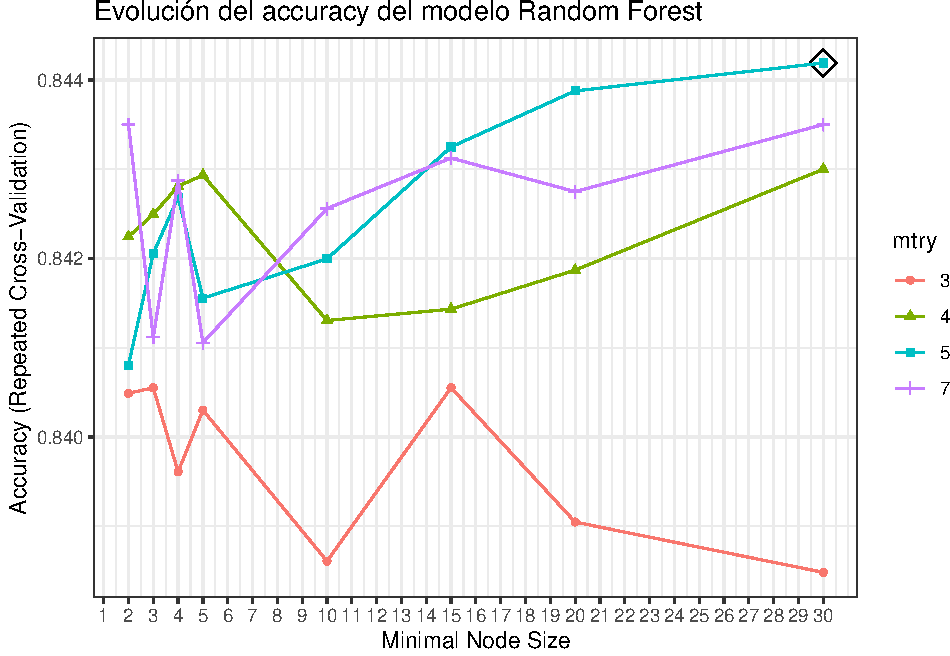
\includegraphics{analisis_de_muchos_modelos_files/figure-latex/unnamed-chunk-24-1.pdf}

\hypertarget{modelar-5}{%
\subsection{Modelar}\label{modelar-5}}

El mejor modelo determinado con los hiperparmétros queda guardado y se
ejecuta nuevamente obteniendo un Accuracy del 84.3\% en entrenamiento.

\begin{lstlisting}
## Ranger result
## 
## Call:
##  ranger::ranger(dependent.variable.name = ".outcome", data = x,      mtry = min(param$mtry, ncol(x)), min.node.size = param$min.node.size,      splitrule = as.character(param$splitrule), write.forest = TRUE,      probability = classProbs, ...) 
## 
## Type:                             Classification 
## Number of trees:                  500 
## Sample size:                      3191 
## Number of independent variables:  24 
## Mtry:                             5 
## Target node size:                 30 
## Variable importance mode:         none 
## Splitrule:                        gini 
## OOB prediction error:             15.70 %
\end{lstlisting}

\begin{table}[!h]

\caption{\label{tab:MatrizConf_RandomForest-Train}Matriz de Confusion del metodo: RandomForest-Train }
\centering
\begin{tabular}[t]{lcc}
\toprule
\multicolumn{1}{c}{Prediccion} & \multicolumn{1}{c}{Referencia} & \multicolumn{1}{c}{ } \\
\cmidrule(l{3pt}r{3pt}){1-1} \cmidrule(l{3pt}r{3pt}){2-2}
\rowcolor{black}  \multicolumn{1}{c}{\textcolor{white}{\textbf{ }}} & \multicolumn{1}{c}{\textcolor{white}{\textbf{0}}} & \multicolumn{1}{c}{\textcolor{white}{\textbf{1}}}\\
\midrule
\rowcolor{gray!6}  0 & 1589 & 202\\
1 & 299 & 1101\\
\bottomrule
\end{tabular}
\end{table}

\begin{lstlisting}
## [1] "Accuracy:"
\end{lstlisting}

\begin{lstlisting}
## [1] 0.8429959
\end{lstlisting}

\hypertarget{describir-el-modelo-5}{%
\subsection{Describir el modelo}\label{describir-el-modelo-5}}

se realiza la evaluacion del modelo con el conjunto de Test. En esta
corrida se obtiene un accuracy de 83.3\% que resulta ser el mejor de los
modelos hasta el momento. Muy cerca de los Valores dl entrenamiento por
lo que aparenta ser un modelo bastante robusto.

\begin{table}[!h]

\caption{\label{tab:MatrizConf_rf}Matriz de Confusion del metodo: rf }
\centering
\begin{tabular}[t]{lcc}
\toprule
\multicolumn{1}{c}{Prediccion} & \multicolumn{1}{c}{Referencia} & \multicolumn{1}{c}{ } \\
\cmidrule(l{3pt}r{3pt}){1-1} \cmidrule(l{3pt}r{3pt}){2-2}
\rowcolor{black}  \multicolumn{1}{c}{\textcolor{white}{\textbf{ }}} & \multicolumn{1}{c}{\textcolor{white}{\textbf{0}}} & \multicolumn{1}{c}{\textcolor{white}{\textbf{1}}}\\
\midrule
\rowcolor{gray!6}  0 & 681 & 135\\
1 & 86 & 465\\
\bottomrule
\end{tabular}
\end{table}

\begin{table}[!h]

\caption{\label{tab:metricas_rf}Métricas del metodo: rf }
\centering
\begin{tabular}[t]{cc}
\toprule
\rowcolor{black}  \multicolumn{1}{c}{\textcolor{white}{\textbf{metricas}}} & \multicolumn{1}{c}{\textcolor{white}{\textbf{valor}}}\\
\midrule
\rowcolor{gray!6}  Accuracy & 0.8383321\\
Kappa & 0.6688211\\
\rowcolor{gray!6}  AccuracyLower & 0.8177277\\
AccuracyUpper & 0.8574701\\
\rowcolor{gray!6}  AccuracyNull & 0.5610827\\
\addlinespace
AccuracyPValue & 0.0000000\\
\rowcolor{gray!6}  McnemarPValue & 0.0012430\\
Sensitivity & 0.7750000\\
\rowcolor{gray!6}  Specificity & 0.8878748\\
Pos Pred Value & 0.8439201\\
\addlinespace
\rowcolor{gray!6}  Neg Pred Value & 0.8345588\\
Precision & 0.8439201\\
\rowcolor{gray!6}  Recall & 0.7750000\\
F1 & 0.8079930\\
\rowcolor{gray!6}  Prevalence & 0.4389173\\
\addlinespace
Detection Rate & 0.3401609\\
\rowcolor{gray!6}  Detection Prevalence & 0.4030724\\
Balanced Accuracy & 0.8314374\\
\bottomrule
\end{tabular}
\end{table}

\hypertarget{gradient-boosting}{%
\section{Gradient Boosting}\label{gradient-boosting}}

Boosting es una de las estrategias que hay de ensemble que se pueden
aplicar a muchos métodos, entre ellos los árboles. Boosting ajusta de
forma secuencia múltiples modelos en cadena. Cada nuevo modelo emplea
información del modelo anterior para aprender de sus errores, mejorando
iteración a iteración. Utiliza todos los features.

\hypertarget{determinar-parametros-del-modelo-2}{%
\section{Determinar parametros del
modelo}\label{determinar-parametros-del-modelo-2}}

Estos métodos se caracterizan por tener muchos hiperparámetros y
parámetros. En este caso se utiliza el paquete gbm y dentro de el se
pueden emplear los siguientes:

\begin{itemize}
\item
  n.trees: número de iteraciones del algoritmo de boosting (cantidad de
  modelos que forman el ensemble). Cuanto mas grande, mas riesgo de
  sobreajuste. Se prueban los siguientes valores: 100, 500, 1000, 2000.
\item
  interaction.depth: complejidad de los árboles (cantidad total de
  divisiones que tiene el árbol). Se preuban los sigientes valores: 1,
  5, 9.
\end{itemize}

shrinkage: (learning rate) controla la influencia que tiene cada modelo
sobre el conjunto del ensemble (aprendizaje). Los valores que se
probaron son: 0.001, 0.01, 0.1.

n.minobsinnode: número mínimo de observaciones que debe tener un nodo
para poder ser dividido. Se probaron los siguientes valores: 2, 10, 20.

distribution: determina la función de coste (loss function). Se utiliza
Adaboost.

bag.fraction (subsampling fraction): Si es de 1, se emplea Gradient
Boosting, si es menor que 1, se emplea Stochastic Gradient Boosting. Por
defecto su valor es de 0.5. Se utiliza valor or defecto.

Se genera una grilla que contempla todas las combinaciones posibles de
los valores mencionados anteriormente. Por cada combinación se generan
una cantidad igual a particiones*repeticiones.

Todos los resultados dan muy similar. La combinación de hiperparámetros
por muy poco y en promedio sobrepasa al resto, es: n.trees = 500,
interaction.depth = 9, shrinkage = 0.01 y n.minobsinnode = 10

\begin{lstlisting}
## Stochastic Gradient Boosting 
## 
## 3191 samples
##   24 predictor
##    2 classes: '0', '1' 
## 
## No pre-processing
## Resampling: Cross-Validated (10 fold, repeated 5 times) 
## Summary of sample sizes: 2872, 2872, 2872, 2872, 2872, 2872, ... 
## Resampling results across tuning parameters:
## 
##   shrinkage  interaction.depth  n.minobsinnode  n.trees  Accuracy   Kappa    
##   0.001      1                   2               100     0.5612657  0.0000000
##   0.001      1                   2               500     0.8047620  0.5878274
##   0.001      1                   2              1000     0.8047620  0.5878274
##   0.001      1                   2              2000     0.8047620  0.5878274
##   0.001      1                  10               100     0.5612657  0.0000000
##   0.001      1                  10               500     0.8047620  0.5878274
##   0.001      1                  10              1000     0.8047620  0.5878274
##   0.001      1                  10              2000     0.8047620  0.5878274
##   0.001      1                  20               100     0.5612657  0.0000000
##   0.001      1                  20               500     0.8047620  0.5878274
##   0.001      1                  20              1000     0.8047620  0.5878274
##   0.001      1                  20              2000     0.8047620  0.5878274
##   0.001      5                   2               100     0.5612657  0.0000000
##   0.001      5                   2               500     0.8278913  0.6395202
##   0.001      5                   2              1000     0.8337232  0.6549784
##   0.001      5                   2              2000     0.8387384  0.6678832
##   0.001      5                  10               100     0.5612657  0.0000000
##   0.001      5                  10               500     0.8288315  0.6414994
##   0.001      5                  10              1000     0.8340991  0.6558040
##   0.001      5                  10              2000     0.8389261  0.6683513
##   0.001      5                  20               100     0.5612657  0.0000000
##   0.001      5                  20               500     0.8243819  0.6320036
##   0.001      5                  20              1000     0.8302132  0.6479565
##   0.001      5                  20              2000     0.8391763  0.6688160
##   0.001      9                   2               100     0.5612657  0.0000000
##   0.001      9                   2               500     0.8347876  0.6559761
##   0.001      9                   2              1000     0.8353525  0.6598282
##   0.001      9                   2              2000     0.8407433  0.6725845
##   0.001      9                  10               100     0.5612657  0.0000000
##   0.001      9                  10               500     0.8340357  0.6542666
##   0.001      9                  10              1000     0.8366695  0.6626417
##   0.001      9                  10              2000     0.8408685  0.6728936
##   0.001      9                  20               100     0.5612657  0.0000000
##   0.001      9                  20               500     0.8288960  0.6431253
##   0.001      9                  20              1000     0.8316552  0.6519327
##   0.001      9                  20              2000     0.8415578  0.6743166
##   0.010      1                   2               100     0.8047620  0.5878274
##   0.010      1                   2               500     0.8368556  0.6618984
##   0.010      1                   2              1000     0.8372337  0.6647654
##   0.010      1                   2              2000     0.8389254  0.6688111
##   0.010      1                  10               100     0.8047620  0.5878274
##   0.010      1                  10               500     0.8369187  0.6620006
##   0.010      1                  10              1000     0.8372964  0.6648140
##   0.010      1                  10              2000     0.8383623  0.6676794
##   0.010      1                  20               100     0.8047620  0.5878274
##   0.010      1                  20               500     0.8374205  0.6630755
##   0.010      1                  20              1000     0.8378599  0.6660065
##   0.010      1                  20              2000     0.8381748  0.6673552
##   0.010      5                   2               100     0.8351021  0.6578923
##   0.010      5                   2               500     0.8431248  0.6785828
##   0.010      5                   2              1000     0.8429369  0.6784049
##   0.010      5                   2              2000     0.8423726  0.6774899
##   0.010      5                  10               100     0.8344132  0.6564703
##   0.010      5                  10               500     0.8432502  0.6789331
##   0.010      5                  10              1000     0.8433754  0.6793564
##   0.010      5                  10              2000     0.8419971  0.6768453
##   0.010      5                  20               100     0.8291475  0.6456523
##   0.010      5                  20               500     0.8416203  0.6754546
##   0.010      5                  20              1000     0.8411193  0.6748054
##   0.010      5                  20              2000     0.8393646  0.6712945
##   0.010      9                   2               100     0.8357921  0.6607389
##   0.010      9                   2               500     0.8426238  0.6777710
##   0.010      9                   2              1000     0.8421844  0.6771109
##   0.010      9                   2              2000     0.8392384  0.6710705
##   0.010      9                  10               100     0.8369826  0.6632902
##   0.010      9                  10               500     0.8434383  0.6794301
##   0.010      9                  10              1000     0.8418717  0.6765381
##   0.010      9                  10              2000     0.8381738  0.6690680
##   0.010      9                  20               100     0.8324071  0.6535178
##   0.010      9                  20               500     0.8424978  0.6773199
##   0.010      9                  20              1000     0.8395515  0.6715888
##   0.010      9                  20              2000     0.8372957  0.6670963
##   0.100      1                   2               100     0.8375460  0.6654062
##   0.100      1                   2               500     0.8381736  0.6674151
##   0.100      1                   2              1000     0.8332206  0.6574298
##   0.100      1                   2              2000     0.8271411  0.6452658
##   0.100      1                  10               100     0.8374228  0.6653564
##   0.100      1                  10               500     0.8376738  0.6664666
##   0.100      1                  10              1000     0.8326571  0.6562193
##   0.100      1                  10              2000     0.8283950  0.6477774
##   0.100      1                  20               100     0.8373595  0.6651134
##   0.100      1                  20               500     0.8378599  0.6667736
##   0.100      1                  20              1000     0.8341607  0.6593135
##   0.100      1                  20              2000     0.8287702  0.6485384
##   0.100      5                   2               100     0.8429369  0.6784541
##   0.100      5                   2               500     0.8337845  0.6602431
##   0.100      5                   2              1000     0.8309647  0.6544684
##   0.100      5                   2              2000     0.8289581  0.6504733
##   0.100      5                  10               100     0.8418082  0.6764154
##   0.100      5                  10               500     0.8330946  0.6588775
##   0.100      5                  10              1000     0.8305251  0.6536612
##   0.100      5                  10              2000     0.8272678  0.6471267
##   0.100      5                  20               100     0.8407428  0.6740054
##   0.100      5                  20               500     0.8292124  0.6510793
##   0.100      5                  20              1000     0.8295223  0.6517475
##   0.100      5                  20              2000     0.8261381  0.6449844
##   0.100      9                   2               100     0.8411824  0.6750311
##   0.100      9                   2               500     0.8325948  0.6577565
##   0.100      9                   2              1000     0.8311509  0.6547442
##   0.100      9                   2              2000     0.8299600  0.6523510
##   0.100      9                  10               100     0.8393000  0.6712852
##   0.100      9                  10               500     0.8311507  0.6548300
##   0.100      9                  10              1000     0.8304626  0.6535543
##   0.100      9                  10              2000     0.8303997  0.6535886
##   0.100      9                  20               100     0.8389888  0.6707469
##   0.100      9                  20               500     0.8301499  0.6530756
##   0.100      9                  20              1000     0.8270167  0.6467869
##   0.100      9                  20              2000     0.8265772  0.6459417
## 
## Accuracy was used to select the optimal model using the largest value.
## The final values used for the model were n.trees = 500, interaction.depth =
##  9, shrinkage = 0.01 and n.minobsinnode = 10.
\end{lstlisting}

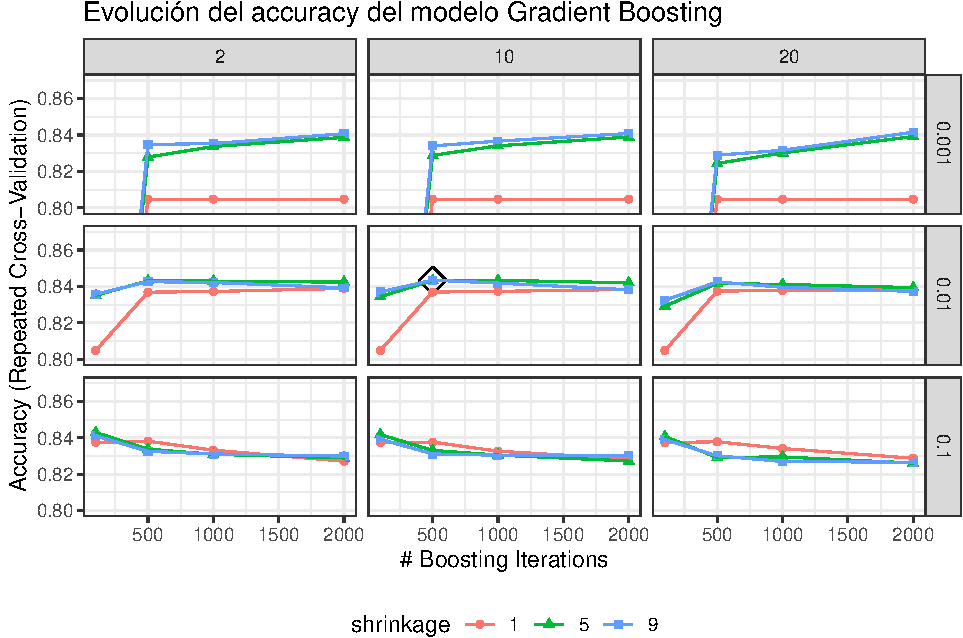
\includegraphics{analisis_de_muchos_modelos_files/figure-latex/unnamed-chunk-28-1.pdf}

\hypertarget{modelar-6}{%
\subsection{Modelar}\label{modelar-6}}

El modelo entrenado tiene un Accuracy del 92\%. El mejor modelo hasta
ahora, aunque puede ser que este un poco sobreajustado.

\begin{lstlisting}
## Stochastic Gradient Boosting 
## 
## 3191 samples
##   24 predictor
##    2 classes: '0', '1' 
## 
## No pre-processing
## Resampling: Cross-Validated (10 fold, repeated 5 times) 
## Summary of sample sizes: 2872, 2872, 2872, 2872, 2872, 2872, ... 
## Resampling results across tuning parameters:
## 
##   shrinkage  interaction.depth  n.minobsinnode  n.trees  Accuracy   Kappa    
##   0.001      1                   2               100     0.5612657  0.0000000
##   0.001      1                   2               500     0.8047620  0.5878274
##   0.001      1                   2              1000     0.8047620  0.5878274
##   0.001      1                   2              2000     0.8047620  0.5878274
##   0.001      1                  10               100     0.5612657  0.0000000
##   0.001      1                  10               500     0.8047620  0.5878274
##   0.001      1                  10              1000     0.8047620  0.5878274
##   0.001      1                  10              2000     0.8047620  0.5878274
##   0.001      1                  20               100     0.5612657  0.0000000
##   0.001      1                  20               500     0.8047620  0.5878274
##   0.001      1                  20              1000     0.8047620  0.5878274
##   0.001      1                  20              2000     0.8047620  0.5878274
##   0.001      5                   2               100     0.5612657  0.0000000
##   0.001      5                   2               500     0.8278913  0.6395202
##   0.001      5                   2              1000     0.8337232  0.6549784
##   0.001      5                   2              2000     0.8387384  0.6678832
##   0.001      5                  10               100     0.5612657  0.0000000
##   0.001      5                  10               500     0.8288315  0.6414994
##   0.001      5                  10              1000     0.8340991  0.6558040
##   0.001      5                  10              2000     0.8389261  0.6683513
##   0.001      5                  20               100     0.5612657  0.0000000
##   0.001      5                  20               500     0.8243819  0.6320036
##   0.001      5                  20              1000     0.8302132  0.6479565
##   0.001      5                  20              2000     0.8391763  0.6688160
##   0.001      9                   2               100     0.5612657  0.0000000
##   0.001      9                   2               500     0.8347876  0.6559761
##   0.001      9                   2              1000     0.8353525  0.6598282
##   0.001      9                   2              2000     0.8407433  0.6725845
##   0.001      9                  10               100     0.5612657  0.0000000
##   0.001      9                  10               500     0.8340357  0.6542666
##   0.001      9                  10              1000     0.8366695  0.6626417
##   0.001      9                  10              2000     0.8408685  0.6728936
##   0.001      9                  20               100     0.5612657  0.0000000
##   0.001      9                  20               500     0.8288960  0.6431253
##   0.001      9                  20              1000     0.8316552  0.6519327
##   0.001      9                  20              2000     0.8415578  0.6743166
##   0.010      1                   2               100     0.8047620  0.5878274
##   0.010      1                   2               500     0.8368556  0.6618984
##   0.010      1                   2              1000     0.8372337  0.6647654
##   0.010      1                   2              2000     0.8389254  0.6688111
##   0.010      1                  10               100     0.8047620  0.5878274
##   0.010      1                  10               500     0.8369187  0.6620006
##   0.010      1                  10              1000     0.8372964  0.6648140
##   0.010      1                  10              2000     0.8383623  0.6676794
##   0.010      1                  20               100     0.8047620  0.5878274
##   0.010      1                  20               500     0.8374205  0.6630755
##   0.010      1                  20              1000     0.8378599  0.6660065
##   0.010      1                  20              2000     0.8381748  0.6673552
##   0.010      5                   2               100     0.8351021  0.6578923
##   0.010      5                   2               500     0.8431248  0.6785828
##   0.010      5                   2              1000     0.8429369  0.6784049
##   0.010      5                   2              2000     0.8423726  0.6774899
##   0.010      5                  10               100     0.8344132  0.6564703
##   0.010      5                  10               500     0.8432502  0.6789331
##   0.010      5                  10              1000     0.8433754  0.6793564
##   0.010      5                  10              2000     0.8419971  0.6768453
##   0.010      5                  20               100     0.8291475  0.6456523
##   0.010      5                  20               500     0.8416203  0.6754546
##   0.010      5                  20              1000     0.8411193  0.6748054
##   0.010      5                  20              2000     0.8393646  0.6712945
##   0.010      9                   2               100     0.8357921  0.6607389
##   0.010      9                   2               500     0.8426238  0.6777710
##   0.010      9                   2              1000     0.8421844  0.6771109
##   0.010      9                   2              2000     0.8392384  0.6710705
##   0.010      9                  10               100     0.8369826  0.6632902
##   0.010      9                  10               500     0.8434383  0.6794301
##   0.010      9                  10              1000     0.8418717  0.6765381
##   0.010      9                  10              2000     0.8381738  0.6690680
##   0.010      9                  20               100     0.8324071  0.6535178
##   0.010      9                  20               500     0.8424978  0.6773199
##   0.010      9                  20              1000     0.8395515  0.6715888
##   0.010      9                  20              2000     0.8372957  0.6670963
##   0.100      1                   2               100     0.8375460  0.6654062
##   0.100      1                   2               500     0.8381736  0.6674151
##   0.100      1                   2              1000     0.8332206  0.6574298
##   0.100      1                   2              2000     0.8271411  0.6452658
##   0.100      1                  10               100     0.8374228  0.6653564
##   0.100      1                  10               500     0.8376738  0.6664666
##   0.100      1                  10              1000     0.8326571  0.6562193
##   0.100      1                  10              2000     0.8283950  0.6477774
##   0.100      1                  20               100     0.8373595  0.6651134
##   0.100      1                  20               500     0.8378599  0.6667736
##   0.100      1                  20              1000     0.8341607  0.6593135
##   0.100      1                  20              2000     0.8287702  0.6485384
##   0.100      5                   2               100     0.8429369  0.6784541
##   0.100      5                   2               500     0.8337845  0.6602431
##   0.100      5                   2              1000     0.8309647  0.6544684
##   0.100      5                   2              2000     0.8289581  0.6504733
##   0.100      5                  10               100     0.8418082  0.6764154
##   0.100      5                  10               500     0.8330946  0.6588775
##   0.100      5                  10              1000     0.8305251  0.6536612
##   0.100      5                  10              2000     0.8272678  0.6471267
##   0.100      5                  20               100     0.8407428  0.6740054
##   0.100      5                  20               500     0.8292124  0.6510793
##   0.100      5                  20              1000     0.8295223  0.6517475
##   0.100      5                  20              2000     0.8261381  0.6449844
##   0.100      9                   2               100     0.8411824  0.6750311
##   0.100      9                   2               500     0.8325948  0.6577565
##   0.100      9                   2              1000     0.8311509  0.6547442
##   0.100      9                   2              2000     0.8299600  0.6523510
##   0.100      9                  10               100     0.8393000  0.6712852
##   0.100      9                  10               500     0.8311507  0.6548300
##   0.100      9                  10              1000     0.8304626  0.6535543
##   0.100      9                  10              2000     0.8303997  0.6535886
##   0.100      9                  20               100     0.8389888  0.6707469
##   0.100      9                  20               500     0.8301499  0.6530756
##   0.100      9                  20              1000     0.8270167  0.6467869
##   0.100      9                  20              2000     0.8265772  0.6459417
## 
## Accuracy was used to select the optimal model using the largest value.
## The final values used for the model were n.trees = 500, interaction.depth =
##  9, shrinkage = 0.01 and n.minobsinnode = 10.
\end{lstlisting}

\begin{table}[!h]

\caption{\label{tab:MatrizConf_GradientBoosting-Train}Matriz de Confusion del metodo: GradientBoosting-Train }
\centering
\begin{tabular}[t]{lcc}
\toprule
\multicolumn{1}{c}{Prediccion} & \multicolumn{1}{c}{Referencia} & \multicolumn{1}{c}{ } \\
\cmidrule(l{3pt}r{3pt}){1-1} \cmidrule(l{3pt}r{3pt}){2-2}
\rowcolor{black}  \multicolumn{1}{c}{\textcolor{white}{\textbf{ }}} & \multicolumn{1}{c}{\textcolor{white}{\textbf{0}}} & \multicolumn{1}{c}{\textcolor{white}{\textbf{1}}}\\
\midrule
\rowcolor{gray!6}  0 & 1631 & 242\\
1 & 160 & 1158\\
\bottomrule
\end{tabular}
\end{table}

\begin{table}[!h]

\caption{\label{tab:metricas_GradientBoosting-Train}Métricas del metodo: GradientBoosting-Train }
\centering
\begin{tabular}[t]{cc}
\toprule
\rowcolor{black}  \multicolumn{1}{c}{\textcolor{white}{\textbf{metricas}}} & \multicolumn{1}{c}{\textcolor{white}{\textbf{valor}}}\\
\midrule
\rowcolor{gray!6}  Accuracy & 0.8740207\\
Kappa & 0.7425548\\
\rowcolor{gray!6}  AccuracyLower & 0.8620072\\
AccuracyUpper & 0.8853438\\
\rowcolor{gray!6}  AccuracyNull & 0.5612661\\
\addlinespace
AccuracyPValue & 0.0000000\\
\rowcolor{gray!6}  McnemarPValue & 0.0000535\\
Sensitivity & 0.8271429\\
\rowcolor{gray!6}  Specificity & 0.9106644\\
Pos Pred Value & 0.8786039\\
\addlinespace
\rowcolor{gray!6}  Neg Pred Value & 0.8707955\\
Precision & 0.8786039\\
\rowcolor{gray!6}  Recall & 0.8271429\\
F1 & 0.8520971\\
\rowcolor{gray!6}  Prevalence & 0.4387339\\
\addlinespace
Detection Rate & 0.3628956\\
\rowcolor{gray!6}  Detection Prevalence & 0.4130367\\
Balanced Accuracy & 0.8689036\\
\bottomrule
\end{tabular}
\end{table}

\hypertarget{describir-el-modelo-6}{%
\subsection{Describir el modelo}\label{describir-el-modelo-6}}

Se evalua el modelo anteiror con el conjunto de Test. Como se observa y
se habia mencionado anteirormente, el modelo evaluado en el conjunto de
test tiene un Accuracy de 83.83\%. Mayor que el promedio del
entrenamiento y menor que el obtenido usando los mejores paramentros con
todo el conjunto de train sin validación.

\begin{table}[!h]

\caption{\label{tab:MatrizConf_boosting}Matriz de Confusion del metodo: boosting }
\centering
\begin{tabular}[t]{lcc}
\toprule
\multicolumn{1}{c}{Prediccion} & \multicolumn{1}{c}{Referencia} & \multicolumn{1}{c}{ } \\
\cmidrule(l{3pt}r{3pt}){1-1} \cmidrule(l{3pt}r{3pt}){2-2}
\rowcolor{black}  \multicolumn{1}{c}{\textcolor{white}{\textbf{ }}} & \multicolumn{1}{c}{\textcolor{white}{\textbf{0}}} & \multicolumn{1}{c}{\textcolor{white}{\textbf{1}}}\\
\midrule
\rowcolor{gray!6}  0 & 678 & 135\\
1 & 89 & 465\\
\bottomrule
\end{tabular}
\end{table}

\begin{table}[!h]

\caption{\label{tab:metricas_boosting}Métricas del metodo: boosting }
\centering
\begin{tabular}[t]{cc}
\toprule
\rowcolor{black}  \multicolumn{1}{c}{\textcolor{white}{\textbf{metricas}}} & \multicolumn{1}{c}{\textcolor{white}{\textbf{valor}}}\\
\midrule
\rowcolor{gray!6}  Accuracy & 0.8361375\\
Kappa & 0.6645097\\
\rowcolor{gray!6}  AccuracyLower & 0.8154319\\
AccuracyUpper & 0.8553864\\
\rowcolor{gray!6}  AccuracyNull & 0.5610827\\
\addlinespace
AccuracyPValue & 0.0000000\\
\rowcolor{gray!6}  McnemarPValue & 0.0026411\\
Sensitivity & 0.7750000\\
\rowcolor{gray!6}  Specificity & 0.8839635\\
Pos Pred Value & 0.8393502\\
\addlinespace
\rowcolor{gray!6}  Neg Pred Value & 0.8339483\\
Precision & 0.8393502\\
\rowcolor{gray!6}  Recall & 0.7750000\\
F1 & 0.8058925\\
\rowcolor{gray!6}  Prevalence & 0.4389173\\
\addlinespace
Detection Rate & 0.3401609\\
\rowcolor{gray!6}  Detection Prevalence & 0.4052670\\
Balanced Accuracy & 0.8294817\\
\bottomrule
\end{tabular}
\end{table}

\hypertarget{svm}{%
\section{SVM}\label{svm}}

Este algoritmo se basa en la separacion de las clases con hiperplanos y
utilizando kernels para aumentar las dimensiones.

\hypertarget{determinar-parametros-del-modelo-3}{%
\subsection{Determinar parametros del
modelo}\label{determinar-parametros-del-modelo-3}}

Se utiliza el paquete kernlab que tiene 2 hiperparámetros:

\begin{itemize}
\item
  sigma: coeficiente del kernel radial. Se preuban los valores: 0.001,
  0.01, 0.1, 0.5, 1.
\item
  C: penalización por violaciones del margen del hiperplano. se preuabn
  los valores: 1 , 20, 50, 100, 200, 500, 700.
\end{itemize}

Los mejores resultados a traves de las iteraciones de los modelos
generados fue con los valores: sigma = 0.001 y C = 100. Los mismos se
contrastan con los valores de Accuracy obtenidos en cada modelo y cuya
evolución puede verse en el grafico x.

\begin{lstlisting}
## Support Vector Machines with Radial Basis Function Kernel 
## 
## 3191 samples
##   24 predictor
##    2 classes: '0', '1' 
## 
## No pre-processing
## Resampling: Cross-Validated (10 fold, repeated 5 times) 
## Summary of sample sizes: 2872, 2872, 2872, 2872, 2872, 2872, ... 
## Resampling results across tuning parameters:
## 
##   sigma  C    Accuracy   Kappa    
##   0.001    1  0.8153017  0.6159483
##   0.001   20  0.8330995  0.6535084
##   0.001   50  0.8349150  0.6578038
##   0.001  100  0.8379236  0.6647011
##   0.001  200  0.8376738  0.6646719
##   0.001  500  0.8369214  0.6638295
##   0.001  700  0.8361060  0.6623453
##   0.010    1  0.8280848  0.6440551
##   0.010   20  0.8312802  0.6525438
##   0.010   50  0.8330335  0.6568089
##   0.010  100  0.8296479  0.6507086
##   0.010  200  0.8297102  0.6512823
##   0.010  500  0.8191179  0.6302330
##   0.010  700  0.8152939  0.6227724
##   0.100    1  0.8194978  0.6283111
##   0.100   20  0.7936720  0.5791574
##   0.100   50  0.7867766  0.5657027
##   0.100  100  0.7825137  0.5573009
##   0.100  200  0.7791299  0.5504630
##   0.100  500  0.7768135  0.5457997
##   0.100  700  0.7747461  0.5416849
##   0.500    1  0.7430247  0.4530058
##   0.500   20  0.7467847  0.4666903
##   0.500   50  0.7472236  0.4676572
##   0.500  100  0.7475366  0.4683001
##   0.500  200  0.7467220  0.4665594
##   0.500  500  0.7467220  0.4665594
##   0.500  700  0.7467220  0.4665594
##   1.000    1  0.6673754  0.2693606
##   1.000   20  0.6806009  0.3050287
##   1.000   50  0.6804126  0.3046084
##   1.000  100  0.6804126  0.3046084
##   1.000  200  0.6804126  0.3046084
##   1.000  500  0.6804126  0.3046084
##   1.000  700  0.6804126  0.3046084
## 
## Accuracy was used to select the optimal model using the largest value.
## The final values used for the model were sigma = 0.001 and C = 100.
\end{lstlisting}

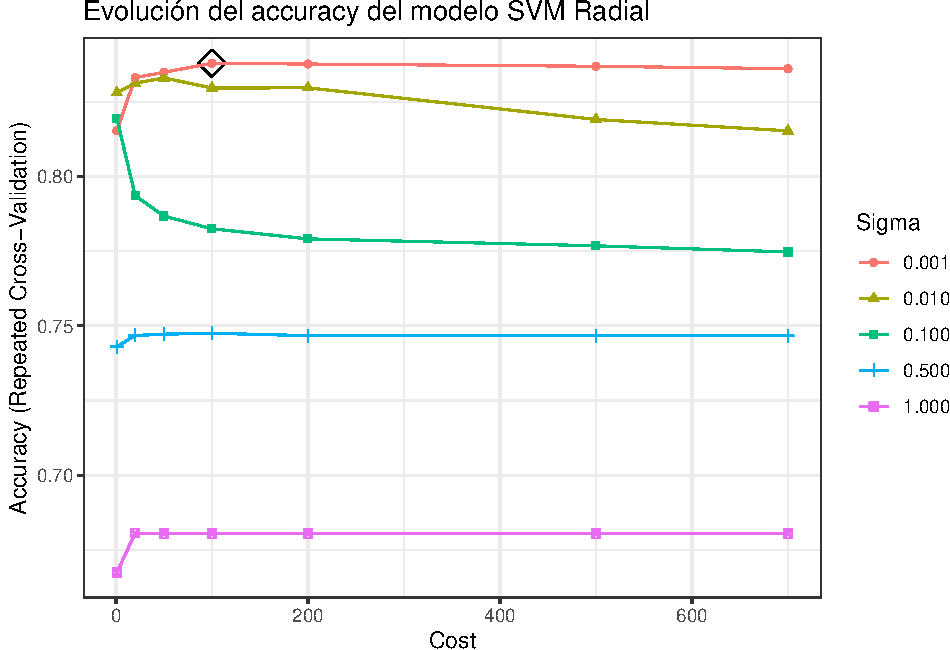
\includegraphics{analisis_de_muchos_modelos_files/figure-latex/unnamed-chunk-32-1.pdf}

\hypertarget{modelar-7}{%
\subsection{Modelar}\label{modelar-7}}

En entrenamiento se consigue un Accuracy de 83.79\% (con validation) y
85.11\% sin validation.

\begin{lstlisting}
## Support Vector Machine object of class "ksvm" 
## 
## SV type: C-svc  (classification) 
##  parameter : cost C = 100 
## 
## Gaussian Radial Basis kernel function. 
##  Hyperparameter : sigma =  0.001 
## 
## Number of Support Vectors : 1227 
## 
## Objective Function Value : -113728.8 
## Training error : 0.148856
\end{lstlisting}

\begin{lstlisting}
## [1] 0.851144
\end{lstlisting}

\begin{table}[!h]

\caption{\label{tab:MatrizConf_SVMradial-Train}Matriz de Confusion del metodo: SVMradial-Train }
\centering
\begin{tabular}[t]{lcc}
\toprule
\multicolumn{1}{c}{Prediccion} & \multicolumn{1}{c}{Referencia} & \multicolumn{1}{c}{ } \\
\cmidrule(l{3pt}r{3pt}){1-1} \cmidrule(l{3pt}r{3pt}){2-2}
\rowcolor{black}  \multicolumn{1}{c}{\textcolor{white}{\textbf{ }}} & \multicolumn{1}{c}{\textcolor{white}{\textbf{0}}} & \multicolumn{1}{c}{\textcolor{white}{\textbf{1}}}\\
\midrule
\rowcolor{gray!6}  0 & 1668 & 352\\
1 & 123 & 1048\\
\bottomrule
\end{tabular}
\end{table}

\begin{table}[!h]

\caption{\label{tab:metricas_SVMradial-Train}Métricas del metodo: SVMradial-Train }
\centering
\begin{tabular}[t]{cc}
\toprule
\rowcolor{black}  \multicolumn{1}{c}{\textcolor{white}{\textbf{metricas}}} & \multicolumn{1}{c}{\textcolor{white}{\textbf{valor}}}\\
\midrule
\rowcolor{gray!6}  Accuracy & 0.8511438\\
Kappa & 0.6922549\\
\rowcolor{gray!6}  AccuracyLower & 0.8383158\\
AccuracyUpper & 0.8633246\\
\rowcolor{gray!6}  AccuracyNull & 0.5612661\\
\addlinespace
AccuracyPValue & 0.0000000\\
\rowcolor{gray!6}  McnemarPValue & 0.0000000\\
Sensitivity & 0.7485714\\
\rowcolor{gray!6}  Specificity & 0.9313233\\
Pos Pred Value & 0.8949616\\
\addlinespace
\rowcolor{gray!6}  Neg Pred Value & 0.8257426\\
Precision & 0.8949616\\
\rowcolor{gray!6}  Recall & 0.7485714\\
F1 & 0.8152470\\
\rowcolor{gray!6}  Prevalence & 0.4387339\\
\addlinespace
Detection Rate & 0.3284237\\
\rowcolor{gray!6}  Detection Prevalence & 0.3669696\\
Balanced Accuracy & 0.8399474\\
\bottomrule
\end{tabular}
\end{table}

\#\#Descripción del modelo

Evaluando en el conjinto de Test se obtiene 84.2\% Accuracy.

\begin{table}[!h]

\caption{\label{tab:MatrizConf_SVMradial}Matriz de Confusion del metodo: SVMradial }
\centering
\begin{tabular}[t]{lcc}
\toprule
\multicolumn{1}{c}{Prediccion} & \multicolumn{1}{c}{Referencia} & \multicolumn{1}{c}{ } \\
\cmidrule(l{3pt}r{3pt}){1-1} \cmidrule(l{3pt}r{3pt}){2-2}
\rowcolor{black}  \multicolumn{1}{c}{\textcolor{white}{\textbf{ }}} & \multicolumn{1}{c}{\textcolor{white}{\textbf{0}}} & \multicolumn{1}{c}{\textcolor{white}{\textbf{1}}}\\
\midrule
\rowcolor{gray!6}  0 & 709 & 158\\
1 & 58 & 442\\
\bottomrule
\end{tabular}
\end{table}

\begin{table}[!h]

\caption{\label{tab:metricas_SVMradial}Métricas del metodo: SVMradial }
\centering
\begin{tabular}[t]{cc}
\toprule
\rowcolor{black}  \multicolumn{1}{c}{\textcolor{white}{\textbf{metricas}}} & \multicolumn{1}{c}{\textcolor{white}{\textbf{valor}}}\\
\midrule
\rowcolor{gray!6}  Accuracy & 0.8419898\\
Kappa & 0.6732633\\
\rowcolor{gray!6}  AccuracyLower & 0.8215568\\
AccuracyUpper & 0.8609401\\
\rowcolor{gray!6}  AccuracyNull & 0.5610827\\
\addlinespace
AccuracyPValue & 0.0000000\\
\rowcolor{gray!6}  McnemarPValue & 0.0000000\\
Sensitivity & 0.7366667\\
\rowcolor{gray!6}  Specificity & 0.9243807\\
Pos Pred Value & 0.8840000\\
\addlinespace
\rowcolor{gray!6}  Neg Pred Value & 0.8177624\\
Precision & 0.8840000\\
\rowcolor{gray!6}  Recall & 0.7366667\\
F1 & 0.8036364\\
\rowcolor{gray!6}  Prevalence & 0.4389173\\
\addlinespace
Detection Rate & 0.3233358\\
\rowcolor{gray!6}  Detection Prevalence & 0.3657644\\
Balanced Accuracy & 0.8305237\\
\bottomrule
\end{tabular}
\end{table}

\hypertarget{modelos-con-dataset-de-variables-reducido}{%
\section{Modelos con Dataset de variables
Reducido}\label{modelos-con-dataset-de-variables-reducido}}

Se pueden utilizar todas las variables, pero scmo se mencionó
anteriormente durante el entrenamiento se comprobaron mejores resultados
con datasets con menos variables. En este caso son 10 variables:

{[}1{]} ``ciclo\_lectivo\_de\_cursada'' ``tipo\_de\_aprobacion\_libre''
``Turno\_Noche''\\
{[}4{]} ``tipo\_de\_aprobacion\_no\_firmo'' ``Aprobado''
``Turno\_Tarde''\\
{[}7{]} ``Nota\_max\_prom'' ``tipo\_de\_aprobacion\_firmo''
``Turno\_Manana''\\
{[}10{]} ``cant\_resursada\_regular''

Por lo que se seleccionaron 3 métodos, para realizar todo el proceso
anterior nuevamente pero solamene teniendo en cuenta estos predictores.
de esta forma y evaluandolo con el conjunto de Test se comprobará que es
mejor.

Los modelos seleccionados para estas pruebas son: Regresión logística,
RandomForest y SVM.

\hypertarget{determinar-paruxe1metros-1}{%
\subsection{Determinar parámetros}\label{determinar-paruxe1metros-1}}

Las grillas de preubas de parámetros es igual para cada modelo que los
mencionados anteriormente las secciones de cada modelo por separado.

Se detallan los nuevos parámetros óptimos encontrados: RandomForest mtry
= 3, splitrule = gini y min.node.size = 30 Reg\_logistica (sin
parametros) SVM sigma = 0.01 y C = 700

\begin{lstlisting}
## [1] "RandomForest"  "Reg_logistica" "SVM"
\end{lstlisting}

\begin{lstlisting}
## $RandomForest
## Random Forest 
## 
## 3191 samples
##   10 predictor
##    2 classes: '0', '1' 
## 
## No pre-processing
## Resampling: Cross-Validated (5 fold, repeated 8 times) 
## Summary of sample sizes: 2553, 2553, 2552, 2553, 2553, 2553, ... 
## Resampling results across tuning parameters:
## 
##   mtry  min.node.size  Accuracy   Kappa    
##   3      2             0.8402566  0.6729637
##   3      3             0.8399044  0.6721908
##   3      4             0.8398650  0.6721515
##   3      5             0.8401388  0.6727699
##   3     10             0.8411571  0.6748184
##   3     15             0.8418232  0.6763003
##   3     20             0.8428417  0.6784827
##   3     30             0.8434285  0.6796168
##   4      2             0.8389243  0.6702716
##   4      3             0.8380234  0.6683855
##   4      4             0.8389249  0.6702389
##   4      5             0.8390034  0.6703180
##   4     10             0.8414709  0.6754611
##   4     15             0.8410398  0.6745944
##   4     20             0.8419796  0.6766335
##   4     30             0.8432330  0.6791114
##   5      2             0.8372407  0.6668464
##   5      3             0.8370831  0.6665059
##   5      4             0.8391985  0.6708436
##   5      5             0.8367308  0.6658576
##   5     10             0.8395504  0.6715448
##   5     15             0.8409218  0.6743952
##   5     20             0.8414701  0.6756383
##   5     30             0.8426070  0.6778691
##   7      2             0.8357903  0.6640102
##   7      3             0.8361824  0.6647902
##   7      4             0.8354773  0.6634469
##   7      5             0.8361047  0.6645979
##   7     10             0.8371221  0.6667474
##   7     15             0.8380230  0.6686637
##   7     20             0.8396293  0.6719409
##   7     30             0.8401771  0.6729758
## 
## Tuning parameter 'splitrule' was held constant at a value of gini
## Accuracy was used to select the optimal model using the largest value.
## The final values used for the model were mtry = 3, splitrule = gini
##  and min.node.size = 30.
## 
## $Reg_logistica
## Generalized Linear Model 
## 
## 3191 samples
##   10 predictor
##    2 classes: '0', '1' 
## 
## No pre-processing
## Resampling: Cross-Validated (5 fold, repeated 8 times) 
## Summary of sample sizes: 2553, 2553, 2552, 2553, 2553, 2553, ... 
## Resampling results:
## 
##   Accuracy   Kappa    
##   0.8313254  0.6508567
\end{lstlisting}

\hypertarget{modelar-8}{%
\subsection{Modelar}\label{modelar-8}}

Los valores de Accuracy obtenidos en entrenamiento:

Random Forest 0.8434285 (con validation) 0.8442495 (usando todo train)
Reg\_logistica 0.8313254 0.8345

\begin{lstlisting}
##     predicted
## true    0    1
##    0 1589  202
##    1  295 1105
\end{lstlisting}

\begin{lstlisting}
## [1] 0.8442495
\end{lstlisting}

\begin{lstlisting}
## 
## Call:  NULL
## 
## Coefficients:
##                 (Intercept)     ciclo_lectivo_de_cursada  
##                     0.35119                     -3.13263  
##    tipo_de_aprobacion_libre                  Turno_Noche  
##                     0.74772                     -0.32733  
## tipo_de_aprobacion_no_firmo                     Aprobado  
##                     0.61234                     -0.57555  
##                 Turno_Tarde                Nota_max_prom  
##                    -0.24499                      0.18274  
##    tipo_de_aprobacion_firmo                 Turno_Manana  
##                    -0.06436                     -0.43394  
##      cant_resursada_regular  
##                    -0.04067  
## 
## Degrees of Freedom: 3190 Total (i.e. Null);  3180 Residual
## Null Deviance:       4376 
## Residual Deviance: 2330  AIC: 2352
\end{lstlisting}

\begin{lstlisting}
## [1] RandomForest  Reg_logistica
## Levels: RandomForest Reg_logistica
\end{lstlisting}

\textbackslash{}begin\{table\}{[}!h{]}

\textbackslash{}caption\{\label{tab:MatrizConf_Reg_logistica-Training}Matriz
de Confusion del metodo: Reg\_logistica-Training \} \centering

\begin{tabular}[t]{lcc}
\toprule
\multicolumn{1}{c}{Prediccion} & \multicolumn{1}{c}{Referencia} & \multicolumn{1}{c}{ } \\
\cmidrule(l{3pt}r{3pt}){1-1} \cmidrule(l{3pt}r{3pt}){2-2}
\rowcolor{black}  \multicolumn{1}{c}{\textcolor{white}{\textbf{ }}} & \multicolumn{1}{c}{\textcolor{white}{\textbf{0}}} & \multicolumn{1}{c}{\textcolor{white}{\textbf{1}}}\\
\midrule
\rowcolor{gray!6}  0 & 1651 & 388\\
1 & 140 & 1012\\
\bottomrule
\end{tabular}

\textbackslash{}end\{table\}

\textbackslash{}begin\{table\}{[}!h{]}

\textbackslash{}caption\{\label{tab:metricas_Reg_logistica-Training}Métricas
del metodo: Reg\_logistica-Training \} \centering

\begin{tabular}[t]{cc}
\toprule
\rowcolor{black}  \multicolumn{1}{c}{\textcolor{white}{\textbf{metricas}}} & \multicolumn{1}{c}{\textcolor{white}{\textbf{valor}}}\\
\midrule
\rowcolor{gray!6}  Accuracy & 0.8345346\\
Kappa & 0.6574003\\
\rowcolor{gray!6}  AccuracyLower & 0.8211795\\
AccuracyUpper & 0.8472735\\
\rowcolor{gray!6}  AccuracyNull & 0.5612661\\
\addlinespace
AccuracyPValue & 0.0000000\\
\rowcolor{gray!6}  McnemarPValue & 0.0000000\\
Sensitivity & 0.7228571\\
\rowcolor{gray!6}  Specificity & 0.9218314\\
Pos Pred Value & 0.8784722\\
\addlinespace
\rowcolor{gray!6}  Neg Pred Value & 0.8097106\\
Precision & 0.8784722\\
\rowcolor{gray!6}  Recall & 0.7228571\\
F1 & 0.7931034\\
\rowcolor{gray!6}  Prevalence & 0.4387339\\
\addlinespace
Detection Rate & 0.3171420\\
\rowcolor{gray!6}  Detection Prevalence & 0.3610154\\
Balanced Accuracy & 0.8223443\\
\bottomrule
\end{tabular}

\textbackslash{}end\{table\}

\hypertarget{describir-el-modelo-7}{%
\subsection{describir el modelo}\label{describir-el-modelo-7}}

con Test

\begin{lstlisting}
## [1] 1367
\end{lstlisting}

\begin{table}[!h]

\caption{\label{tab:MatrizConf_RandomForest}Matriz de Confusion del metodo: RandomForest }
\centering
\begin{tabular}[t]{lcc}
\toprule
\multicolumn{1}{c}{Prediccion} & \multicolumn{1}{c}{Referencia} & \multicolumn{1}{c}{ } \\
\cmidrule(l{3pt}r{3pt}){1-1} \cmidrule(l{3pt}r{3pt}){2-2}
\rowcolor{black}  \multicolumn{1}{c}{\textcolor{white}{\textbf{ }}} & \multicolumn{1}{c}{\textcolor{white}{\textbf{0}}} & \multicolumn{1}{c}{\textcolor{white}{\textbf{1}}}\\
\midrule
\rowcolor{gray!6}  0 & 684 & 135\\
1 & 83 & 465\\
\bottomrule
\end{tabular}
\end{table}

\begin{table}[!h]

\caption{\label{tab:metricas_RandomForest}Métricas del metodo: RandomForest }
\centering
\begin{tabular}[t]{cc}
\toprule
\rowcolor{black}  \multicolumn{1}{c}{\textcolor{white}{\textbf{metricas}}} & \multicolumn{1}{c}{\textcolor{white}{\textbf{valor}}}\\
\midrule
\rowcolor{gray!6}  Accuracy & 0.8405267\\
Kappa & 0.6731372\\
\rowcolor{gray!6}  AccuracyLower & 0.8200248\\
AccuracyUpper & 0.8595526\\
\rowcolor{gray!6}  AccuracyNull & 0.5610827\\
\addlinespace
AccuracyPValue & 0.0000000\\
\rowcolor{gray!6}  McnemarPValue & 0.0005520\\
Sensitivity & 0.7750000\\
\rowcolor{gray!6}  Specificity & 0.8917862\\
Pos Pred Value & 0.8485401\\
\addlinespace
\rowcolor{gray!6}  Neg Pred Value & 0.8351648\\
Precision & 0.8485401\\
\rowcolor{gray!6}  Recall & 0.7750000\\
F1 & 0.8101045\\
\rowcolor{gray!6}  Prevalence & 0.4389173\\
\addlinespace
Detection Rate & 0.3401609\\
\rowcolor{gray!6}  Detection Prevalence & 0.4008778\\
Balanced Accuracy & 0.8333931\\
\bottomrule
\end{tabular}
\end{table}

\begin{lstlisting}
## [1] 1367
\end{lstlisting}

\textbackslash{}begin\{table\}{[}!h{]}

\textbackslash{}caption\{\label{tab:MatrizConf_Reg_logistica}Matriz de
Confusion del metodo: Reg\_logistica \} \centering

\begin{tabular}[t]{lcc}
\toprule
\multicolumn{1}{c}{Prediccion} & \multicolumn{1}{c}{Referencia} & \multicolumn{1}{c}{ } \\
\cmidrule(l{3pt}r{3pt}){1-1} \cmidrule(l{3pt}r{3pt}){2-2}
\rowcolor{black}  \multicolumn{1}{c}{\textcolor{white}{\textbf{ }}} & \multicolumn{1}{c}{\textcolor{white}{\textbf{0}}} & \multicolumn{1}{c}{\textcolor{white}{\textbf{1}}}\\
\midrule
\rowcolor{gray!6}  0 & 684 & 135\\
1 & 83 & 465\\
\bottomrule
\end{tabular}

\textbackslash{}end\{table\}

\textbackslash{}begin\{table\}{[}!h{]}

\textbackslash{}caption\{\label{tab:metricas_Reg_logistica}Métricas del
metodo: Reg\_logistica \} \centering

\begin{tabular}[t]{cc}
\toprule
\rowcolor{black}  \multicolumn{1}{c}{\textcolor{white}{\textbf{metricas}}} & \multicolumn{1}{c}{\textcolor{white}{\textbf{valor}}}\\
\midrule
\rowcolor{gray!6}  Accuracy & 0.8405267\\
Kappa & 0.6731372\\
\rowcolor{gray!6}  AccuracyLower & 0.8200248\\
AccuracyUpper & 0.8595526\\
\rowcolor{gray!6}  AccuracyNull & 0.5610827\\
\addlinespace
AccuracyPValue & 0.0000000\\
\rowcolor{gray!6}  McnemarPValue & 0.0005520\\
Sensitivity & 0.7750000\\
\rowcolor{gray!6}  Specificity & 0.8917862\\
Pos Pred Value & 0.8485401\\
\addlinespace
\rowcolor{gray!6}  Neg Pred Value & 0.8351648\\
Precision & 0.8485401\\
\rowcolor{gray!6}  Recall & 0.7750000\\
F1 & 0.8101045\\
\rowcolor{gray!6}  Prevalence & 0.4389173\\
\addlinespace
Detection Rate & 0.3401609\\
\rowcolor{gray!6}  Detection Prevalence & 0.4008778\\
Balanced Accuracy & 0.8333931\\
\bottomrule
\end{tabular}

\textbackslash{}end\{table\}

\hypertarget{modelos-con-dataset-sin-variable-ciclo_lectivo_de_cursada}{%
\section{Modelos con Dataset sin variable
ciclo\_lectivo\_de\_cursada}\label{modelos-con-dataset-sin-variable-ciclo_lectivo_de_cursada}}

En este caso, se generan algunos modelos pero usando el dataset sin la
variable que mayor relevancia tomaba para los modelos anteriores (sin
``ciclo\_lectivo\_de\_cursada'')

Los modelos seleccionados para estas pruebas son: Regresión logística,
RandomForest, knn y GradientBoosting.

\begin{lstlisting}
## [1] "RandomForest"  "Reg_logistica"
\end{lstlisting}

\begin{lstlisting}
## [1] "GradienBoosting_3"
\end{lstlisting}

\begin{lstlisting}
## $GradienBoosting_3
## Stochastic Gradient Boosting 
## 
## 3191 samples
##    9 predictor
##    2 classes: '0', '1' 
## 
## No pre-processing
## Resampling: Cross-Validated (5 fold, repeated 8 times) 
## Summary of sample sizes: 2553, 2553, 2552, 2553, 2553, 2553, ... 
## Resampling results across tuning parameters:
## 
##   shrinkage  interaction.depth  n.minobsinnode  n.trees  Accuracy   Kappa    
##   0.001      1                   2               500     0.7097712  0.4135733
##   0.001      1                   2              1000     0.7181152  0.4322519
##   0.001      1                   2              2000     0.7348411  0.4614070
##   0.001      1                   5               500     0.7094969  0.4127321
##   0.001      1                   5              1000     0.7183108  0.4326995
##   0.001      1                   5              2000     0.7348411  0.4614168
##   0.001      1                  15               500     0.7103196  0.4149736
##   0.001      1                  15              1000     0.7181937  0.4323522
##   0.001      1                  15              2000     0.7342147  0.4601123
##   0.001      2                   2               500     0.7268511  0.4302101
##   0.001      2                   2              1000     0.7403639  0.4677604
##   0.001      2                   2              2000     0.7507051  0.4912349
##   0.001      2                   5               500     0.7266942  0.4299188
##   0.001      2                   5              1000     0.7407165  0.4684953
##   0.001      2                   5              2000     0.7508621  0.4915558
##   0.001      2                  15               500     0.7258714  0.4281312
##   0.001      2                  15              1000     0.7410688  0.4693392
##   0.001      2                  15              2000     0.7510579  0.4920116
##   0.010      1                   2               500     0.7536438  0.4987455
##   0.010      1                   2              1000     0.7632409  0.5186205
##   0.010      1                   2              2000     0.7691957  0.5305265
##   0.010      1                   5               500     0.7540755  0.4995368
##   0.010      1                   5              1000     0.7623002  0.5166580
##   0.010      1                   5              2000     0.7693916  0.5309110
##   0.010      1                  15               500     0.7536834  0.4988552
##   0.010      1                  15              1000     0.7626528  0.5174907
##   0.010      1                  15              2000     0.7699792  0.5320814
##   0.010      2                   2               500     0.7643778  0.5204404
##   0.010      2                   2              1000     0.7695096  0.5310391
##   0.010      2                   2              2000     0.7729178  0.5380343
##   0.010      2                   5               500     0.7635939  0.5190155
##   0.010      2                   5              1000     0.7713117  0.5348366
##   0.010      2                   5              2000     0.7735832  0.5393915
##   0.010      2                  15               500     0.7642208  0.5201417
##   0.010      2                  15              1000     0.7715465  0.5351816
##   0.010      2                  15              2000     0.7742495  0.5406675
##   0.100      1                   2               500     0.7713894  0.5346826
##   0.100      1                   2              1000     0.7680200  0.5274630
##   0.100      1                   2              2000     0.7628498  0.5167840
##   0.100      1                   5               500     0.7702921  0.5325393
##   0.100      1                   5              1000     0.7672365  0.5258047
##   0.100      1                   5              2000     0.7620663  0.5151777
##   0.100      1                  15               500     0.7716241  0.5350175
##   0.100      1                  15              1000     0.7677855  0.5270363
##   0.100      1                  15              2000     0.7620665  0.5150443
##   0.100      2                   2               500     0.7703708  0.5329246
##   0.100      2                   2              1000     0.7659064  0.5238798
##   0.100      2                   2              2000     0.7614013  0.5147818
##   0.100      2                   5               500     0.7675517  0.5270057
##   0.100      2                   5              1000     0.7628513  0.5178061
##   0.100      2                   5              2000     0.7576412  0.5070964
##   0.100      2                  15               500     0.7681004  0.5282994
##   0.100      2                  15              1000     0.7647714  0.5214325
##   0.100      2                  15              2000     0.7587369  0.5092640
## 
## Accuracy was used to select the optimal model using the largest value.
## The final values used for the model were n.trees = 2000, interaction.depth =
##  2, shrinkage = 0.01 and n.minobsinnode = 15.
\end{lstlisting}

\begin{lstlisting}
## $RandomForest
## Random Forest 
## 
## 3191 samples
##    9 predictor
##    2 classes: '0', '1' 
## 
## No pre-processing
## Resampling: Cross-Validated (5 fold, repeated 8 times) 
## Summary of sample sizes: 2553, 2553, 2552, 2553, 2553, 2553, ... 
## Resampling results across tuning parameters:
## 
##   mtry  min.node.size  Accuracy   Kappa    
##   3      2             0.7671206  0.5282249
##   3      3             0.7665719  0.5271329
##   3      4             0.7672766  0.5285668
##   3      5             0.7666903  0.5274872
##   3     10             0.7700196  0.5341778
##   3     15             0.7695101  0.5334912
##   3     20             0.7697845  0.5340891
##   3     30             0.7720178  0.5387246
##   4      2             0.7646133  0.5231270
##   4      3             0.7664932  0.5268484
##   4      4             0.7659055  0.5259800
##   4      5             0.7656712  0.5253449
##   4     10             0.7676689  0.5295171
##   4     15             0.7699800  0.5343340
##   4     20             0.7693140  0.5329868
##   4     30             0.7708810  0.5363738
##   5      2             0.7640269  0.5217434
##   5      3             0.7630079  0.5197385
##   5      4             0.7646127  0.5229645
##   5      5             0.7644957  0.5229746
##   5     10             0.7671606  0.5285420
##   5     15             0.7682956  0.5307551
##   5     20             0.7683344  0.5309660
##   5     30             0.7699800  0.5343229
##   7      2             0.7609303  0.5154202
##   7      3             0.7621059  0.5177764
##   7      4             0.7632023  0.5202340
##   7      5             0.7644169  0.5226701
##   7     10             0.7637510  0.5214020
##   7     15             0.7654751  0.5251842
##   7     20             0.7668063  0.5278189
##   7     30             0.7682571  0.5308204
## 
## Tuning parameter 'splitrule' was held constant at a value of gini
## Accuracy was used to select the optimal model using the largest value.
## The final values used for the model were mtry = 3, splitrule = gini
##  and min.node.size = 30.
## 
## $Reg_logistica
## Generalized Linear Model 
## 
## 3191 samples
##    9 predictor
##    2 classes: '0', '1' 
## 
## No pre-processing
## Resampling: Cross-Validated (5 fold, repeated 8 times) 
## Summary of sample sizes: 2553, 2553, 2552, 2553, 2553, 2553, ... 
## Resampling results:
## 
##   Accuracy   Kappa    
##   0.7532915  0.5033037
\end{lstlisting}

\hypertarget{determinar-paruxe1metros-2}{%
\subsection{Determinar parámetros}\label{determinar-paruxe1metros-2}}

Las grillas de preubas de parámetros es igual para cada modelo que los
mencionados anteriormente las secciones de cada modelo por separado.

Se detallan los nuevos parámetros óptimos encontrados: RandomForest mtry
= 3, splitrule = gini and min.node.size = 30 Reg\_logistica (sin
parametros) gbm n.trees = 2000, interaction.depth = 2, shrinkage = 0.01
y n.minobsinnode = 15

\begin{lstlisting}
## $RandomForest
## Random Forest 
## 
## 3191 samples
##    9 predictor
##    2 classes: '0', '1' 
## 
## No pre-processing
## Resampling: Cross-Validated (5 fold, repeated 8 times) 
## Summary of sample sizes: 2553, 2553, 2552, 2553, 2553, 2553, ... 
## Resampling results across tuning parameters:
## 
##   mtry  min.node.size  Accuracy   Kappa    
##   3      2             0.7671206  0.5282249
##   3      3             0.7665719  0.5271329
##   3      4             0.7672766  0.5285668
##   3      5             0.7666903  0.5274872
##   3     10             0.7700196  0.5341778
##   3     15             0.7695101  0.5334912
##   3     20             0.7697845  0.5340891
##   3     30             0.7720178  0.5387246
##   4      2             0.7646133  0.5231270
##   4      3             0.7664932  0.5268484
##   4      4             0.7659055  0.5259800
##   4      5             0.7656712  0.5253449
##   4     10             0.7676689  0.5295171
##   4     15             0.7699800  0.5343340
##   4     20             0.7693140  0.5329868
##   4     30             0.7708810  0.5363738
##   5      2             0.7640269  0.5217434
##   5      3             0.7630079  0.5197385
##   5      4             0.7646127  0.5229645
##   5      5             0.7644957  0.5229746
##   5     10             0.7671606  0.5285420
##   5     15             0.7682956  0.5307551
##   5     20             0.7683344  0.5309660
##   5     30             0.7699800  0.5343229
##   7      2             0.7609303  0.5154202
##   7      3             0.7621059  0.5177764
##   7      4             0.7632023  0.5202340
##   7      5             0.7644169  0.5226701
##   7     10             0.7637510  0.5214020
##   7     15             0.7654751  0.5251842
##   7     20             0.7668063  0.5278189
##   7     30             0.7682571  0.5308204
## 
## Tuning parameter 'splitrule' was held constant at a value of gini
## Accuracy was used to select the optimal model using the largest value.
## The final values used for the model were mtry = 3, splitrule = gini
##  and min.node.size = 30.
## 
## $Reg_logistica
## Generalized Linear Model 
## 
## 3191 samples
##    9 predictor
##    2 classes: '0', '1' 
## 
## No pre-processing
## Resampling: Cross-Validated (5 fold, repeated 8 times) 
## Summary of sample sizes: 2553, 2553, 2552, 2553, 2553, 2553, ... 
## Resampling results:
## 
##   Accuracy   Kappa    
##   0.7532915  0.5033037
\end{lstlisting}

\begin{lstlisting}
## $GradienBoosting_3
## Stochastic Gradient Boosting 
## 
## 3191 samples
##    9 predictor
##    2 classes: '0', '1' 
## 
## No pre-processing
## Resampling: Cross-Validated (5 fold, repeated 8 times) 
## Summary of sample sizes: 2553, 2553, 2552, 2553, 2553, 2553, ... 
## Resampling results across tuning parameters:
## 
##   shrinkage  interaction.depth  n.minobsinnode  n.trees  Accuracy   Kappa    
##   0.001      1                   2               500     0.7097712  0.4135733
##   0.001      1                   2              1000     0.7181152  0.4322519
##   0.001      1                   2              2000     0.7348411  0.4614070
##   0.001      1                   5               500     0.7094969  0.4127321
##   0.001      1                   5              1000     0.7183108  0.4326995
##   0.001      1                   5              2000     0.7348411  0.4614168
##   0.001      1                  15               500     0.7103196  0.4149736
##   0.001      1                  15              1000     0.7181937  0.4323522
##   0.001      1                  15              2000     0.7342147  0.4601123
##   0.001      2                   2               500     0.7268511  0.4302101
##   0.001      2                   2              1000     0.7403639  0.4677604
##   0.001      2                   2              2000     0.7507051  0.4912349
##   0.001      2                   5               500     0.7266942  0.4299188
##   0.001      2                   5              1000     0.7407165  0.4684953
##   0.001      2                   5              2000     0.7508621  0.4915558
##   0.001      2                  15               500     0.7258714  0.4281312
##   0.001      2                  15              1000     0.7410688  0.4693392
##   0.001      2                  15              2000     0.7510579  0.4920116
##   0.010      1                   2               500     0.7536438  0.4987455
##   0.010      1                   2              1000     0.7632409  0.5186205
##   0.010      1                   2              2000     0.7691957  0.5305265
##   0.010      1                   5               500     0.7540755  0.4995368
##   0.010      1                   5              1000     0.7623002  0.5166580
##   0.010      1                   5              2000     0.7693916  0.5309110
##   0.010      1                  15               500     0.7536834  0.4988552
##   0.010      1                  15              1000     0.7626528  0.5174907
##   0.010      1                  15              2000     0.7699792  0.5320814
##   0.010      2                   2               500     0.7643778  0.5204404
##   0.010      2                   2              1000     0.7695096  0.5310391
##   0.010      2                   2              2000     0.7729178  0.5380343
##   0.010      2                   5               500     0.7635939  0.5190155
##   0.010      2                   5              1000     0.7713117  0.5348366
##   0.010      2                   5              2000     0.7735832  0.5393915
##   0.010      2                  15               500     0.7642208  0.5201417
##   0.010      2                  15              1000     0.7715465  0.5351816
##   0.010      2                  15              2000     0.7742495  0.5406675
##   0.100      1                   2               500     0.7713894  0.5346826
##   0.100      1                   2              1000     0.7680200  0.5274630
##   0.100      1                   2              2000     0.7628498  0.5167840
##   0.100      1                   5               500     0.7702921  0.5325393
##   0.100      1                   5              1000     0.7672365  0.5258047
##   0.100      1                   5              2000     0.7620663  0.5151777
##   0.100      1                  15               500     0.7716241  0.5350175
##   0.100      1                  15              1000     0.7677855  0.5270363
##   0.100      1                  15              2000     0.7620665  0.5150443
##   0.100      2                   2               500     0.7703708  0.5329246
##   0.100      2                   2              1000     0.7659064  0.5238798
##   0.100      2                   2              2000     0.7614013  0.5147818
##   0.100      2                   5               500     0.7675517  0.5270057
##   0.100      2                   5              1000     0.7628513  0.5178061
##   0.100      2                   5              2000     0.7576412  0.5070964
##   0.100      2                  15               500     0.7681004  0.5282994
##   0.100      2                  15              1000     0.7647714  0.5214325
##   0.100      2                  15              2000     0.7587369  0.5092640
## 
## Accuracy was used to select the optimal model using the largest value.
## The final values used for the model were n.trees = 2000, interaction.depth =
##  2, shrinkage = 0.01 and n.minobsinnode = 15.
\end{lstlisting}

\hypertarget{modelar-9}{%
\subsection{Modelar}\label{modelar-9}}

Los valores de Accuracy obtenidos en entrenamiento:

Random Forest 0.7720178 (con validation) 0.7731119 (usando todo train)
Reg\_logistica 0.7532915 0.7558759 gbm 0.7510579 0.7919148

\begin{lstlisting}
##     predicted
## true    0    1
##    0 1407  384
##    1  340 1060
\end{lstlisting}

\begin{lstlisting}
## [1] 0.7731119
\end{lstlisting}

\begin{lstlisting}
## 
## Call:  NULL
## 
## Coefficients:
##                 (Intercept)     tipo_de_aprobacion_libre  
##                    -0.54964                      1.02282  
##                 Turno_Noche  tipo_de_aprobacion_no_firmo  
##                    -0.94356                      0.77148  
##                    Aprobado                  Turno_Tarde  
##                    -0.90726                     -0.67434  
##               Nota_max_prom     tipo_de_aprobacion_firmo  
##                     0.02305                      0.66797  
##                Turno_Manana       cant_resursada_regular  
##                    -0.97639                     -0.05740  
## 
## Degrees of Freedom: 3190 Total (i.e. Null);  3181 Residual
## Null Deviance:       4376 
## Residual Deviance: 3336  AIC: 3356
\end{lstlisting}

\begin{lstlisting}
## [1] RandomForest_3  Reg_Logistica_3
## Levels: RandomForest_3 Reg_Logistica_3
\end{lstlisting}

\textbackslash{}begin\{table\}{[}!h{]}

\textbackslash{}caption\{\label{tab:MatrizConf_Reg_logistica_3-Training}Matriz
de Confusion del metodo: Reg\_logistica\_3-Training \} \centering

\begin{tabular}[t]{lcc}
\toprule
\multicolumn{1}{c}{Prediccion} & \multicolumn{1}{c}{Referencia} & \multicolumn{1}{c}{ } \\
\cmidrule(l{3pt}r{3pt}){1-1} \cmidrule(l{3pt}r{3pt}){2-2}
\rowcolor{black}  \multicolumn{1}{c}{\textcolor{white}{\textbf{ }}} & \multicolumn{1}{c}{\textcolor{white}{\textbf{0}}} & \multicolumn{1}{c}{\textcolor{white}{\textbf{1}}}\\
\midrule
\rowcolor{gray!6}  0 & 1343 & 331\\
1 & 448 & 1069\\
\bottomrule
\end{tabular}

\textbackslash{}end\{table\}

\textbackslash{}begin\{table\}{[}!h{]}

\textbackslash{}caption\{\label{tab:metricas_Reg_logistica_3-Training}Métricas
del metodo: Reg\_logistica\_3-Training \} \centering

\begin{tabular}[t]{cc}
\toprule
\rowcolor{black}  \multicolumn{1}{c}{\textcolor{white}{\textbf{metricas}}} & \multicolumn{1}{c}{\textcolor{white}{\textbf{valor}}}\\
\midrule
\rowcolor{gray!6}  Accuracy & 0.7558759\\
Kappa & 0.5087905\\
\rowcolor{gray!6}  AccuracyLower & 0.7405843\\
AccuracyUpper & 0.7706971\\
\rowcolor{gray!6}  AccuracyNull & 0.5612661\\
\addlinespace
AccuracyPValue & 0.0000000\\
\rowcolor{gray!6}  McnemarPValue & 0.0000324\\
Sensitivity & 0.7635714\\
\rowcolor{gray!6}  Specificity & 0.7498604\\
Pos Pred Value & 0.7046803\\
\addlinespace
\rowcolor{gray!6}  Neg Pred Value & 0.8022700\\
Precision & 0.7046803\\
\rowcolor{gray!6}  Recall & 0.7635714\\
F1 & 0.7329448\\
\rowcolor{gray!6}  Prevalence & 0.4387339\\
\addlinespace
Detection Rate & 0.3350047\\
\rowcolor{gray!6}  Detection Prevalence & 0.4753996\\
Balanced Accuracy & 0.7567159\\
\bottomrule
\end{tabular}

\textbackslash{}end\{table\}

\begin{lstlisting}
## A gradient boosted model with adaboost loss function.
## 2000 iterations were performed.
## There were 9 predictors of which 9 had non-zero influence.
\end{lstlisting}

\begin{lstlisting}
## [1] GBM_3
## Levels: GBM_3
\end{lstlisting}

\textbackslash{}begin\{table\}{[}!h{]}

\textbackslash{}caption\{\label{tab:MatrizConf_GBM_3-Training}Matriz de
Confusion del metodo: GBM\_3-Training \} \centering

\begin{tabular}[t]{lcc}
\toprule
\multicolumn{1}{c}{Prediccion} & \multicolumn{1}{c}{Referencia} & \multicolumn{1}{c}{ } \\
\cmidrule(l{3pt}r{3pt}){1-1} \cmidrule(l{3pt}r{3pt}){2-2}
\rowcolor{black}  \multicolumn{1}{c}{\textcolor{white}{\textbf{ }}} & \multicolumn{1}{c}{\textcolor{white}{\textbf{0}}} & \multicolumn{1}{c}{\textcolor{white}{\textbf{1}}}\\
\midrule
\rowcolor{gray!6}  0 & 1465 & 338\\
1 & 326 & 1062\\
\bottomrule
\end{tabular}

\textbackslash{}end\{table\}

\textbackslash{}begin\{table\}{[}!h{]}

\textbackslash{}caption\{\label{tab:metricas_GBM_3-Training}Métricas del
metodo: GBM\_3-Training \} \centering

\begin{tabular}[t]{cc}
\toprule
\rowcolor{black}  \multicolumn{1}{c}{\textcolor{white}{\textbf{metricas}}} & \multicolumn{1}{c}{\textcolor{white}{\textbf{valor}}}\\
\midrule
\rowcolor{gray!6}  Accuracy & 0.7919148\\
Kappa & 0.5770902\\
\rowcolor{gray!6}  AccuracyLower & 0.7774089\\
AccuracyUpper & 0.8058835\\
\rowcolor{gray!6}  AccuracyNull & 0.5612661\\
\addlinespace
AccuracyPValue & 0.0000000\\
\rowcolor{gray!6}  McnemarPValue & 0.6694647\\
Sensitivity & 0.7585714\\
\rowcolor{gray!6}  Specificity & 0.8179788\\
Pos Pred Value & 0.7651297\\
\addlinespace
\rowcolor{gray!6}  Neg Pred Value & 0.8125347\\
Precision & 0.7651297\\
\rowcolor{gray!6}  Recall & 0.7585714\\
F1 & 0.7618364\\
\rowcolor{gray!6}  Prevalence & 0.4387339\\
\addlinespace
Detection Rate & 0.3328110\\
\rowcolor{gray!6}  Detection Prevalence & 0.4349734\\
Balanced Accuracy & 0.7882751\\
\bottomrule
\end{tabular}

\textbackslash{}end\{table\}

\hypertarget{describir-el-modelo-8}{%
\subsection{describir el modelo}\label{describir-el-modelo-8}}

con Test

RandomFores 0.7717630 Reg\_Logistica 0.7439649 gbm 0.6949525

\textbackslash{}begin\{table\}{[}!h{]}

\textbackslash{}caption\{\label{tab:MatrizConf_RandomForest_3}Matriz de
Confusion del metodo: RandomForest\_3 \} \centering

\begin{tabular}[t]{lcc}
\toprule
\multicolumn{1}{c}{Prediccion} & \multicolumn{1}{c}{Referencia} & \multicolumn{1}{c}{ } \\
\cmidrule(l{3pt}r{3pt}){1-1} \cmidrule(l{3pt}r{3pt}){2-2}
\rowcolor{black}  \multicolumn{1}{c}{\textcolor{white}{\textbf{ }}} & \multicolumn{1}{c}{\textcolor{white}{\textbf{0}}} & \multicolumn{1}{c}{\textcolor{white}{\textbf{1}}}\\
\midrule
\rowcolor{gray!6}  0 & 599 & 144\\
1 & 168 & 456\\
\bottomrule
\end{tabular}

\textbackslash{}end\{table\}

\textbackslash{}begin\{table\}{[}!h{]}

\textbackslash{}caption\{\label{tab:metricas_RandomForest_3}Métricas del
metodo: RandomForest\_3 \} \centering

\begin{tabular}[t]{cc}
\toprule
\rowcolor{black}  \multicolumn{1}{c}{\textcolor{white}{\textbf{metricas}}} & \multicolumn{1}{c}{\textcolor{white}{\textbf{valor}}}\\
\midrule
\rowcolor{gray!6}  Accuracy & 0.7717630\\
Kappa & 0.5386193\\
\rowcolor{gray!6}  AccuracyLower & 0.7485776\\
AccuracyUpper & 0.7937739\\
\rowcolor{gray!6}  AccuracyNull & 0.5610827\\
\addlinespace
AccuracyPValue & 0.0000000\\
\rowcolor{gray!6}  McnemarPValue & 0.1928758\\
Sensitivity & 0.7600000\\
\rowcolor{gray!6}  Specificity & 0.7809648\\
Pos Pred Value & 0.7307692\\
\addlinespace
\rowcolor{gray!6}  Neg Pred Value & 0.8061911\\
Precision & 0.7307692\\
\rowcolor{gray!6}  Recall & 0.7600000\\
F1 & 0.7450980\\
\rowcolor{gray!6}  Prevalence & 0.4389173\\
\addlinespace
Detection Rate & 0.3335772\\
\rowcolor{gray!6}  Detection Prevalence & 0.4564740\\
Balanced Accuracy & 0.7704824\\
\bottomrule
\end{tabular}

\textbackslash{}end\{table\}

\textbackslash{}begin\{table\}{[}!h{]}

\textbackslash{}caption\{\label{tab:MatrizConf_Reg_Logistica_3}Matriz de
Confusion del metodo: Reg\_Logistica\_3 \} \centering

\begin{tabular}[t]{lcc}
\toprule
\multicolumn{1}{c}{Prediccion} & \multicolumn{1}{c}{Referencia} & \multicolumn{1}{c}{ } \\
\cmidrule(l{3pt}r{3pt}){1-1} \cmidrule(l{3pt}r{3pt}){2-2}
\rowcolor{black}  \multicolumn{1}{c}{\textcolor{white}{\textbf{ }}} & \multicolumn{1}{c}{\textcolor{white}{\textbf{0}}} & \multicolumn{1}{c}{\textcolor{white}{\textbf{1}}}\\
\midrule
\rowcolor{gray!6}  0 & 574 & 157\\
1 & 193 & 443\\
\bottomrule
\end{tabular}

\textbackslash{}end\{table\}

\textbackslash{}begin\{table\}{[}!h{]}

\textbackslash{}caption\{\label{tab:metricas_Reg_Logistica_3}Métricas
del metodo: Reg\_Logistica\_3 \} \centering

\begin{tabular}[t]{cc}
\toprule
\rowcolor{black}  \multicolumn{1}{c}{\textcolor{white}{\textbf{metricas}}} & \multicolumn{1}{c}{\textcolor{white}{\textbf{valor}}}\\
\midrule
\rowcolor{gray!6}  Accuracy & 0.7439649\\
Kappa & 0.4835451\\
\rowcolor{gray!6}  AccuracyLower & 0.7199541\\
AccuracyUpper & 0.7669222\\
\rowcolor{gray!6}  AccuracyNull & 0.5610827\\
\addlinespace
AccuracyPValue & 0.0000000\\
\rowcolor{gray!6}  McnemarPValue & 0.0613688\\
Sensitivity & 0.7383333\\
\rowcolor{gray!6}  Specificity & 0.7483703\\
Pos Pred Value & 0.6965409\\
\addlinespace
\rowcolor{gray!6}  Neg Pred Value & 0.7852257\\
Precision & 0.6965409\\
\rowcolor{gray!6}  Recall & 0.7383333\\
F1 & 0.7168285\\
\rowcolor{gray!6}  Prevalence & 0.4389173\\
\addlinespace
Detection Rate & 0.3240673\\
\rowcolor{gray!6}  Detection Prevalence & 0.4652524\\
Balanced Accuracy & 0.7433518\\
\bottomrule
\end{tabular}

\textbackslash{}end\{table\}

\textbackslash{}begin\{table\}{[}!h{]}

\textbackslash{}caption\{\label{tab:MatrizConf_GBM_3}Matriz de Confusion
del metodo: GBM\_3 \} \centering

\begin{tabular}[t]{lcc}
\toprule
\multicolumn{1}{c}{Prediccion} & \multicolumn{1}{c}{Referencia} & \multicolumn{1}{c}{ } \\
\cmidrule(l{3pt}r{3pt}){1-1} \cmidrule(l{3pt}r{3pt}){2-2}
\rowcolor{black}  \multicolumn{1}{c}{\textcolor{white}{\textbf{ }}} & \multicolumn{1}{c}{\textcolor{white}{\textbf{0}}} & \multicolumn{1}{c}{\textcolor{white}{\textbf{1}}}\\
\midrule
\rowcolor{gray!6}  0 & 617 & 267\\
1 & 150 & 333\\
\bottomrule
\end{tabular}

\textbackslash{}end\{table\}

\textbackslash{}begin\{table\}{[}!h{]}

\textbackslash{}caption\{\label{tab:metricas_GBM_3}Métricas del metodo:
GBM\_3 \} \centering

\begin{tabular}[t]{cc}
\toprule
\rowcolor{black}  \multicolumn{1}{c}{\textcolor{white}{\textbf{metricas}}} & \multicolumn{1}{c}{\textcolor{white}{\textbf{valor}}}\\
\midrule
\rowcolor{gray!6}  Accuracy & 0.6949525\\
Kappa & 0.3672287\\
\rowcolor{gray!6}  AccuracyLower & 0.6697789\\
AccuracyUpper & 0.7192851\\
\rowcolor{gray!6}  AccuracyNull & 0.5610827\\
\addlinespace
AccuracyPValue & 0.0000000\\
\rowcolor{gray!6}  McnemarPValue & 0.0000000\\
Sensitivity & 0.5550000\\
\rowcolor{gray!6}  Specificity & 0.8044329\\
Pos Pred Value & 0.6894410\\
\addlinespace
\rowcolor{gray!6}  Neg Pred Value & 0.6979638\\
Precision & 0.6894410\\
\rowcolor{gray!6}  Recall & 0.5550000\\
F1 & 0.6149584\\
\rowcolor{gray!6}  Prevalence & 0.4389173\\
\addlinespace
Detection Rate & 0.2435991\\
\rowcolor{gray!6}  Detection Prevalence & 0.3533285\\
Balanced Accuracy & 0.6797164\\
\bottomrule
\end{tabular}

\textbackslash{}end\{table\}

\hypertarget{modelos-que-usan-todas-las-variables-menos-la-mas-importante}{%
\section{modelos que usan todas las variables menos la mas
importante}\label{modelos-que-usan-todas-las-variables-menos-la-mas-importante}}

\hypertarget{comparar-modelos}{%
\section{COMPARAR MODELOS}\label{comparar-modelos}}

para compara modelos se unen los datsets de predicciones

\begin{table}[!h]

\caption{\label{tab:cuadro_comparativo-modelos}Resumen comparativo de algunos los modelos empleados}
\centering
\begin{tabular}[t]{lrr}
\toprule
\rowcolor{black}  \multicolumn{1}{c}{\textcolor{white}{\textbf{object}}} & \multicolumn{1}{c}{\textcolor{white}{\textbf{Test}}} & \multicolumn{1}{c}{\textcolor{white}{\textbf{Training}}}\\
\midrule
\rowcolor{gray!6}  SVMradial & 0.8419898 & 0.8511438\\
RandomForest & 0.8405267 & 0.9100595\\
\rowcolor{gray!6}  rf & 0.8383321 & 0.9194610\\
boosting & 0.8361375 & 0.8740207\\
\rowcolor{gray!6}  logistic & 0.8354060 & 0.8420558\\
\addlinespace
Reg\_logistica & 0.8339429 & 0.8345346\\
\rowcolor{gray!6}  arbol & 0.8324799 & 0.8552178\\
LDA & 0.8266277 & 0.8301473\\
\rowcolor{gray!6}  KNN & 0.8024872 & 0.8182388\\
RandomForest\_5 & 0.7849305 & 0.9674083\\
\addlinespace
\rowcolor{gray!6}  SVM\_5 & 0.7820044 & 0.7988092\\
RandomForest\_3 & 0.7717630 & 0.8686932\\
\rowcolor{gray!6}  Reg\_logistica\_5 & 0.7717630 & 0.7768725\\
C50\_5 & 0.7534748 & 0.8147916\\
\rowcolor{gray!6}  GradienBoosting\_5 & 0.7520117 & 0.7963021\\
\addlinespace
Reg\_Logistica\_3 & 0.7439649 & 0.7558759\\
\bottomrule
\end{tabular}
\end{table}

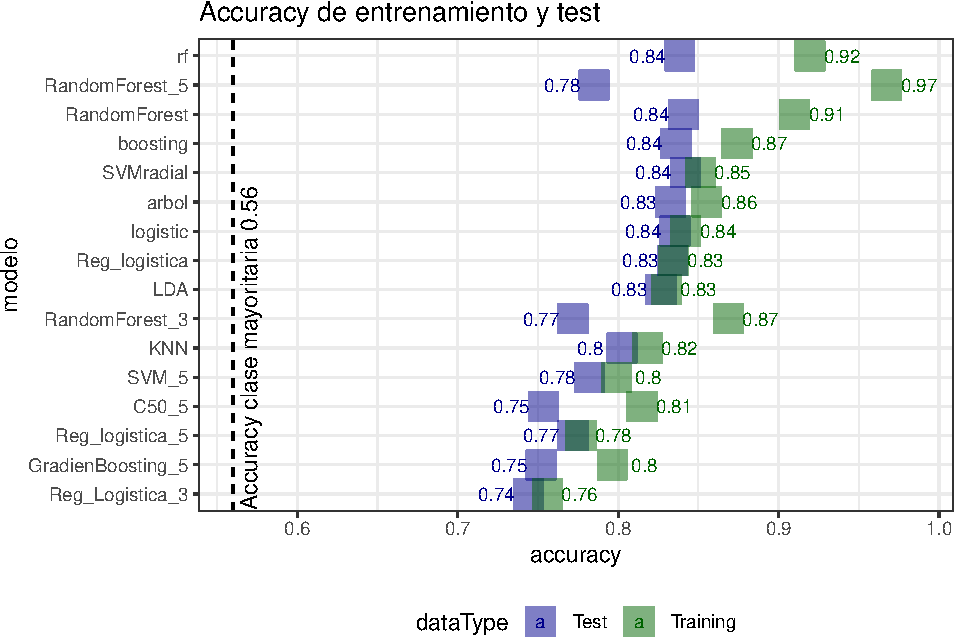
\includegraphics{analisis_de_muchos_modelos_files/figure-latex/unnamed-chunk-53-1.pdf}

\end{document}
